% первая часть

% первая глава

\section{Методы получения трехмерных изображений из двумерных}

В ходе выполнения проекта, главным образом, решается задача преобразования двумерных изображений в трехмерные на мобильных устройствах.

В последние годы заметное место в области преобразования и фильтрации изображений занимает задача преобразования двумерных изображений в трехмерные. На сегодняшний день в мире для этого разработаны различные методики, которые позволяют автоматически создавать так называемые «карты глубины»~\cite{depthMap3} (рисунок ~\ref{fig:s-63}) для двумерных изображений, основываясь на свойствах этого изображение и на некоторых предположениях о характере сцены. 

\begin{figure}[H]
	\centering
	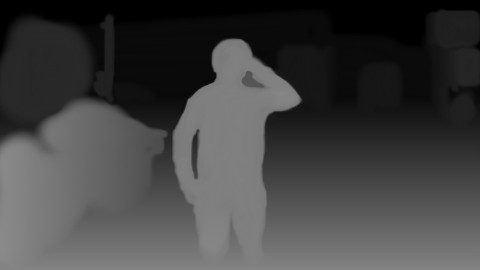
\includegraphics[width=0.7\linewidth]{pics/s-63}
	\caption{карта глубины}
	\label{fig:s-63}
\end{figure} В частности, были проведены исследования следующих методов получения трехмерных изображений из двумерных:

\begin{itemize}
	\item Предположение о том, что изображение имеет линейную перспективу;
	\item Предположение о том, что снимок сделан на открытом пространстве и использование модели рассеяния световых лучей в атмосфере;
	\item Обнаружение теней и восстановление по ним карты глубины;
	\item Обнаружение перекрытий объектов на изображении и используя эту информацию восстановлении карты глубины;
	\item Использование моделей пространственных искажений заданных текстур;
	\item Использование билатеральных симметричных шаблонов;
	\item Использование статистических методов для обучения текстурных шаблонов, на различных расстояниях от объектива и другие методы.
\end{itemize}

Практически все эти методы характеризуются достаточно узким характером сцен, которые могут быть реализованы для преобразования в трехмерное изображение. 

Проведенные предварительные исследования показали, что одним из наиболее перспективных методов преобразования изображений в трехмерные считается метод «дефокусировки», который предполагает, что близкие объекты находятся в фокусе, а более удаленные объекты имеют большее размытие. Используя информацию о размытии той или иной точки на изображении можно предположить о том, насколько далеко она находится от объектива. Используя метод дефокусировки можно построить карту глубины для любой макрофотографии. 

Известные методы получения карты глубины, использующие дефокус удаленных от объектива объектов, основаны на следующей цепочке преобразования изображения~\cite{depthMap1}:

\begin{enumerate} 
	\item Обнаружение краев объектов с использованием фильтра Канни.
	\item Для каждой точки найденного края выполняется оценка расстояния, до нее с использованием гауссовского размытия. Таким образом строится так называемая разреженная карта глубины, которая несет информацию о расстоянии до объектива в некоторых точках изображения. 
	\item Разреженная карта глубины с использованием интерполяции превращается в так называемую «плотную карту глубины», которая уже пригодна для построения трехмерного изображения сцены с любого ракурса. 
\end{enumerate}

Реализация мобильного приложения позволяющего оперативно переводить стандартные фотоизображения в 3D-снимки чрезвычайно актуально и востребовано. С другой стороны, на сегодняшний день имеется определенный научный задел по разработке алгоритмов преобразования 2D -3D. В частности известен ряд различных методик, которые позволяют автоматически создавать «карты глубины» для двумерных изображений, основываясь на свойствах этого изображение, и на некоторых предположениях о характере сцены. Например метод дефокусировки позволяет построить карту глубины фотографии. Вместе с тем информации о программно реализованных в том числе мобильных приложений крайне мало. 

Рассмотренный метод преобразования (см. пункты 1-3) предыдущего раздела страдает двумя существенными недостатками\cite{depthMap2}.

\begin{enumerate}
	\item Разреженная карта глубины получается не всегда гладкой, что приводит к ошибкам последующей интерполяции и, в итоге, к ошибкам в карте глубины. 
	\item Окончательная интерполяция для построения требует больших вычислительных затрат и до последнего времени не имела возможности быть встроенной в мобильные приложения. 
\end{enumerate}

Основываясь на этих двух недостатках существующего метода дефокусировки изображения, требуется провести научное исследование в следующих направлениях:

\begin{enumerate}
	\item Адаптивное сглаживание разреженной карты глубины.  С использованием методов кластеризации краев изображения, в протяженные структуры, глубина точек которых должна подчиняться некоторому закону, а не быть случайной от точки к точке, как в существующем методе. 
	\item Найти способ снижения вычислительных затрат для выполнения двумерной интерполяции при построении плотной карты глубины. 
	\item Нам представляется, что для преобразования двумерного видеоролика в трехмерное представление необходимо разработать методику передачи разреженной карты глубины (с учетом сглаживания) от кадра к кадру. 
\end{enumerate}

Таким образом предлагаемый Проект на сегодняшний день актуален и содержит помимо научной алгоритмической составляющей широкие перспективы коммерциализации.

\section{Технические требования.}

В ходе выполнения проекта будет создана методика количественной оценки достоверности построения карты глубины, которая необходима для корректного преобразования 2D изображения в 3D вид. Эта методика основана на сравнении показаний глубины, полученных в результате работы алгоритмов преобразования 2D –> 3D и достоверных показаний глубины для данной сцены, которые получены в ручном режиме.

Для реализации методики предполагается произвести ручную разметку тестовых цифровых фотографий в количестве не менее 100 штук. Для этого в ручном режиме устанавливаются контрольные точки, с указанием расстояния до них.

Таким образом формируется разреженная карта глубины, с указанием абсолютных значений. Далее, на изображении находится самая дальняя контрольная точка и все расстояния нормируются на расстояние до нее. Таким образом формируется разреженная карта глубины с относительными расстояниями, и, как следствие, (алгоритмически) формируется «эталонная» плотная карта глубины.

Далее, в результате работы различных алгоритмов преобразования изображения из двумерного в трехмерное автоматически вычисляется как разреженная карта глубины для каждого из анализируемых алгоритмов (создаваемого в рамках проекта и конкурирующих аналогов). Далее предполагается вычислять среднеквадратичную ошибку между эталонными значениями для карты глубины и значениями, вычисленными каждым из алгоритмов.

Предполагается, что алгоритм, реализуемый в ходе выполнения проекта даст снижение такой ошибки между вычисленными и эталонными значениями на величину не менее 25\% (ожидаемое значение – порядка 30\%).

Необходимая задача при реализации проекта - адаптация существующего метода преобразования 2D в 3D для использования под управлением операционной системы Android.

В ходе выполнения проекта будут созданы мобильные приложения со следующими характеристиками:

\begin{itemize}
	\item мобильное приложение, функционирующее под управлением операционной системы Android версии не ниже 5.0.
	\item специальных дополнительных требований к аппаратному обеспечению мобильных устройств не предъявляется. Они соответствуют требованиям, накладываемым вышеперечисленными версиями ОС.
	\item мобильные приложения должны функционировать на устройствах с разными размерами экрана от 2.6 до 6 дюймов с разрешениями от 240х320 до 1440х2560 пикселей.
	\item источник данных для конвертирования - файлы в формате jpeg из галереи мобильного устройства или фотография, сделанная штатной фотокамерой мобильного устройства.
	\item мобильные приложения должны обеспечивать конвертацию сделанных фотокамерой изображений при максимальном качестве съемки не менее 10 Мп.
	\item формат данных, в которых сохраняются результаты --- анаглиф файлы (формат jpeg), стерео пара (формат jps), анимированные файлы в формате gif.
	\item ориентировочное время преобразования 2D в 3D не должно превышать 5 секунд.
\end{itemize}

\subsection{Технологические требования}

Создаваемое в рамках проекта мобильное приложение должно функционировать под управлением мобильных операционных систем Android и iOS.

\begin{itemize}
	\item Программное обеспечение должно создаваться в строгом соответствии с модульным принципом.
	\item Программное обеспечение должно быть реализовано в виде <<нативных>> приложений для вышеперечисленных операционных систем.
	\item Ожидаемое время преобразования цифровой фотографии в трехмерный вид не должно превышать 5ти секунд. 
\end{itemize}

Технические требования к аппаратному обеспечению мобильного устройства и ограничения, накладываемые на преобразуемые фотографии, будут уточнены в ходе выполнения проекта.

\section{Разработка концепции и архитектуры мобильных приложений, предназначенных для преобразования 2D в 3D.}
В ходе выполнения работы были рассмотрены различные варианты для создания мобильных приложений, предназначенных для преобразования 2D изображений в 3D вид. При этом рассмотрении учитывалось, что результирующие мобильные приложения должны создаваться под операционные системы Android и iOS, а также то, что один из основных результатов работы приложения с точки зрения конечного пользователя – это возможность публикации созданного 3D-изображения в виде анимированного gif-файла в одном или нескольких аккаунтов в социальных сетях пользователя. Соответственно, можно исходить из предположения о том, что для функционирования приложения в любом случае необходим доступ к сети интернет. Максимальная унификация различных составных частей приложения между собой хотя бы на уровне исходных кодов вне зависимости от целевой платформы (Android или iOS) является дополнительным преимуществом при рассмотрении различных вариантов создания мобильных приложений.

Один из наиболее простых с технической точки зрения вариантов реализации решения, позволяющего преобразовывать 2D файлы в 3D вид, является решение, основанное на создании веб-сервиса, который предоставляет минимально необходимый пользовательский интерфейс для загрузки желаемого файла на сервер, преобразования файла на сервере и, как результат, возможность скачать получившийся файл на устройство пользователя и поделиться этим файлом в социальных сетях. При простоте архитектуры у этого решения есть один существенных недостаток – как правило, такие решения менее удобны и функциональны, чем нативные (native) мобильные приложения, разработанные специально под целевую платформу, на которой они будут функционировать. Поэтому на данном этапе от такого подхода было принято решение отказаться.

Если рассматривать варианты создания нативных мобильных приложений, существует несколько возможных вариантов:

\begin{enumerate}
	\item Использовать наиболее популярные средства разработки и языки программирования для каждой из необходимых мобильных платформ. Создать нативное мобильное приложение, реализующее весь необходимый пользовательский интерфейс, набор сервисных функций. Портировать алгоритм преобразования графического файла из 2D в 3D для локального исполнения на мобильном устройстве. Все необходимые преобразования выполнять локально, на мобильном устройстве. Полученный результат преобразования (анимированный gif) загружать в интернет (социальные сети) по мере его готовности на мобильном устройстве.
	\item Использовать наиболее популярные средства разработки и языки программирования для каждой из необходимых мобильных платформ для создания нативных мобильных приложений только для реализации пользовательского интерфейса и набора сервисных функций. Алгоритм преобразования графического файла из 2D в 3D реализуется в виде серверного модуля, соответственно для преобразования выбранного файла и предварительного просмотра полученных результатов необходимо загрузить этот выбранный файл на сервер. Загрузить полученный результат с сервера и поделиться этим результатом в социальных сетях.
	\item Использовать кроссплатформенное средство разработки мобильных решений Xamarin. Это средство одновременно позволяет создавать iOS, Android и Windows Phone приложения. Реализация алгоритма преобразования графического файла из 2D в 3D модифицируется таким образом, что может быть непосредственно интегрирована в Xamarin-проект. В результате получается единое решение, которое на этапе сборки может быть превращено в полнофункциональное нативное приложение для любой из поддерживаемых платформ --- iOS, Android и Windows Phone. Результирующее решение будет преобразовывать графические файлы из 2D в 3D локально на мобильном устройстве, доступ к интернету необходим только для реализации функции «поделиться созданным 3D-файлом в социальных сетях».
	\item Использовать кроссплатформенное средство разработки мобильных решений Xamarin, но только лишь для создания нативных мобильных приложений. реализующих пользовательский интерфейс и набор сервисных функций. Алгоритм преобразования графического файла из 2D в 3D реализуется в виде серверного модуля, соответственно для преобразования выбранного файла и предварительного просмотра полученных результатов необходимо загрузить этот выбранный файл на сервер. Загрузить полученный результат с сервера и поделиться этим результатом в социальных сетях.
\end{enumerate}

Перед тем, как рассмотреть каждый из приведенных выше вариантов по отдельности, следует отметить, что существующая на сегодняшний день реализация алгоритма преобразования изображений из 2D в 3D вид реализована на языке С++, сборка осуществляется с использованием Microsoft Visual Studio, соответствующее решение имеет существенную зависимость от OpenCV (Open Source Computer Vision Library – это программная библиотека с открытым исходным кодом, реализующая базовые алгоритмы компьютерного зрения, обработки изображений и численных алгоритмов общего назначения. Реализована на C/C++).

Возвращаемся к вышеперечисленным вариантам.

Для варианта №1 для операционной системы Android необходимо:

С использованием Android Studio на языке программирования Java реализовать необходимый пользовательский интерфейс, а также весь необходимый набор сервисных функций. Необходимо адаптировать реализацию алгоритма преобразования графического файла из 2D в 3D для использования под управлением операционной системы Android (реализация на С++). Далее, с использованием механизма The Android Native Development Kit (NDK) необходимо обеспечить вызов кода, написанного на языке С++ из «классического» Android-приложения. 

Для разработки приложений для iOS основным средством разработки является Objective-C. Проведенные предварительные исследования показали, что адаптировать реализацию алгоритма преобразования графического файла из 2D в 3D для использования под управлением операционной системы iOS с разумными усилиями не представляется возможным. Соответственно, вариант №1 является неприемлемым для реализации решения для операционной системы iOS.

Для реализации варианта №2 необходимо:

С использованием наиболее популярных средств разработки и языков программирования для каждой из необходимых мобильных платформ (Java для Android и Objective С для iOS) необходимо создать нативные мобильных приложений для реализации пользовательского интерфейса и набора сервисных функций. Эта задача, в целом, является типовой и принципиальных сложностей не вызывает. Алгоритм преобразования графического файла из 2D в 3D следует реализовать в виде серверного модуля, например, для использования под управлением операционной системы Ubuntu. Это обусловлено тем, что Unix-подобные операционные системы имеют существенно более широкое распространение в Web-серверном окружении, чем Windows-сервера. Основная сложность данной задачи – в сборке и корректном использовании OpenCV библиотеки под Linux, однако аналогичная задача сравнительно недавно была решена коллегами для реализации демонстрационного видеоплеера для использования под операционной системой Ubuntu.

Для реализации варианта №3 необходимо адаптировать алгоритм преобразования графического файла из 2D в 3D таким образом, чтобы он мог быть непосредственно интегрирован в Xamarin-проект (разработка на языке программирования С\#). Проведенные предварительные исследования показали, что реализовать подобный функционал за разумное время с разумными усилиями не представляется возможным.

Вариант №4 основывается на разработке унифицированного решения для всех поддерживаемых мобильных платформ (iOS, Android и Windows Phone) для реализации пользовательского интерфейса и сервисных функций на языке программирования С\#. В части алгоритма преобразования графического файла из 2D в 3D этот вариант полностью аналогичен (точнее даже унифицирован) варианту №2 – должен быть реализован серверный модуль, например, для использования под управлением операционной системы Ubuntu для реализации этого преобразования. И, соответственно, с помощью реализованных на С\# функций выбирается файл для преобразования, отправляется на сервер, там преобразовывается, скачивается обратно для предварительного просмотра полученных результатов, а далее реализуется возможность поделиться полученным результатом в социальных сетях.

На основе проведенного исследования моно сделать следующий вывод. С точки зрения скорости, легкости и качества реализации наиболее перспективными являются варианты №2 и №4. Однако, вариант №4, в силу кроссплатформенности, унифицированности решения для всех поддерживаемых мобильных платформ является более предпочтительным. Соответственно, на реализации этого варианта и будут сосредоточены усилия на самом первом этапе развития проекта. 

Очевидным недостатком подобного решения является существенная его зависимость от скорости и надежности мобильного интернета, а также от доступности конечному пользователю оплаченного траффика. Для обхода этих ограничений предполагается исследовать возможность создания для пользователей ОС Android «самодостаточного» мобильного приложения (вариант №1), которое все необходимые действия, связанные с преобразованием файлов производит непосредственно на мобильном устройстве. Хочется надеяться, что необходимая для этого адаптация алгоритма преобразования графического файла из 2D в 3D для использования под управлением операционной системы Android (после создания реализации этого алгоритма по Ubuntu, основная проблема – возможность использования OpenCV под соответствующую платформу – должна решаться аналогичным образом) не доставит много хлопот.


\section{Анализ существующих продуктов со схожим функционалом} // Дублируется далее
Одной из задач при создании мобильного приложения для преобразования 2D фотографий в 3D вид, является разработка пользовательского интерфейса.

Для достижения этой задачи были проанализированы аналогичные приложения, которые очень популярны на сегодняшний день: Prisma, Pixlr, Candy Camera.

В первую очередь, целью сравнения являлся анализ особенностей пользовательского интерфейса этих приложений. Это обусловлено тем, что, во многом, схема функционирования приложения, которое планируется создать в ходе выполнения проекта, аналогична схеме работы этих приложений. А именно: пользователь делает фотографию при помощи штатной камеры своего смартфона или загружает уже существующее изображение из галереи, отправляет изображение на обработку, просматривает результат и, если результат ему нравится, сохраняет или отправляет получившееся изображение в одну или несколько социальных сетей.

Таким образом можно выделить 4 основных окна приложения:
\begin{enumerate}
	\item Режим камеры, делаем фотографию.
	\item Окно выбора фотографии из галереи.
	\item Окно применения фильтра, смотрим готовый результат.
	\item Окно выбора действий с получившейся фотографией.
\end{enumerate}

\subsection{Prisma}
Проанализировав пользовательский интерфейс первого приложения Prisma (рисунок~\ref{fig:prismaCam}), в режиме камера увидели заметные отличия - это наличие статус бара и возможность переключения между камерой, лентой и профилем в верхней части экрана или свайпом, движением пальца по экрану телефона влево и вправо. Все кнопки расположены удобно и их назначения интуитивно понятны. В галереи показаны все изображения, имеющиеся в смартфоне (рисунок ~\ref{fig:prismaGal}). После применения фильтра есть возможность обрезать фото в нужном соотношении (рисунок ~\ref{fig:prismaProp}).

\begin{figure}[H]
	\centering
	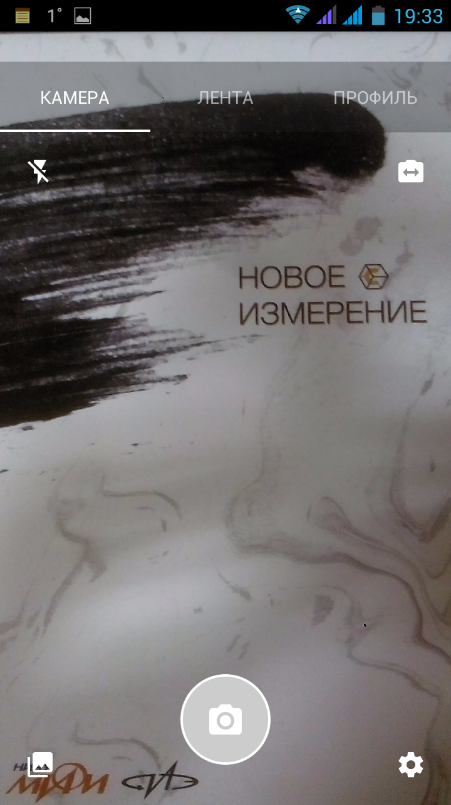
\includegraphics[width=0.3\linewidth]{pics/prismaCam}
	%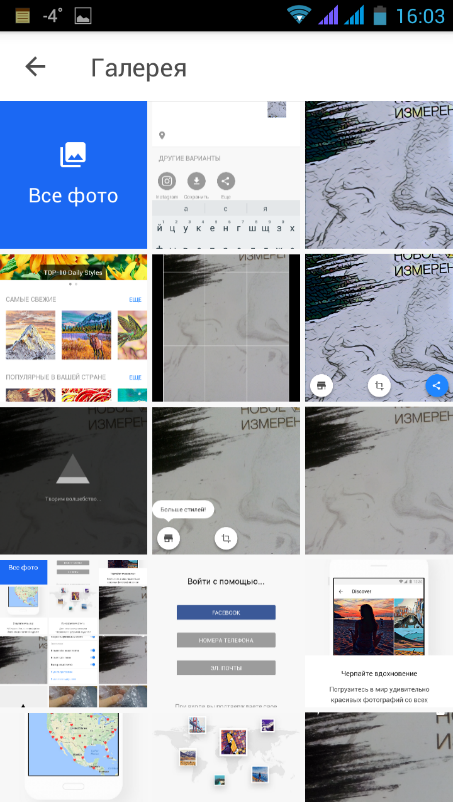
\includegraphics[width=0.3\linewidth]{pics/prismaGal}
	%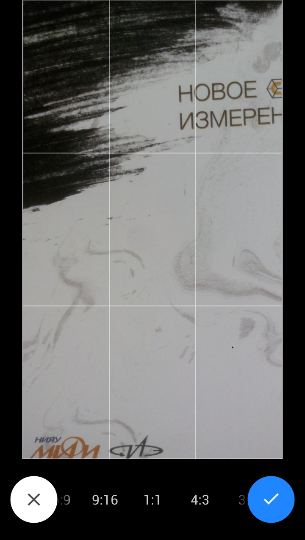
\includegraphics[width=0.3\linewidth]{pics/prismaProp}
	\caption{Prisma, окно с камерой}
	\label{fig:prismaCam}
	\label{fig:prismaGal}
	\label{fig:prismaProp}
\end{figure}

\begin{figure}[H]
	\centering
	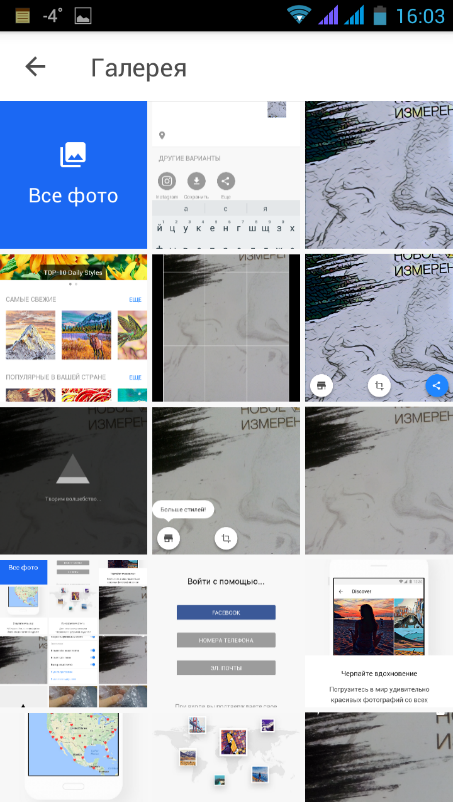
\includegraphics[width=0.3\linewidth]{pics/prismaGal}
	\caption{Prisma, окно с галереей}
	\label{fig:prismaGal}
\end{figure}

\begin{figure}[H]
	\centering
	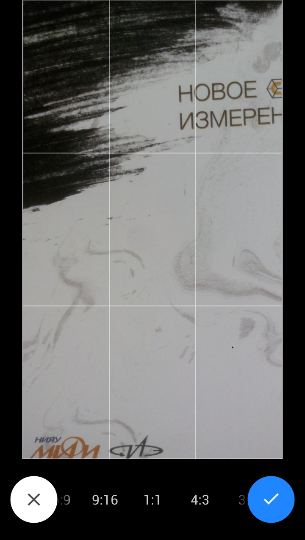
\includegraphics[width=0.3\linewidth]{pics/prismaProp}
	\caption{Prisma, окно выбора пропорции для изображения}
	\label{fig:prismaProp}
\end{figure}

\subsection{Candy Camera}
Проанализировав пользовательский интерфейс приложения Candy Camera (рисунок~\ref{fig:candyCam}), в режиме камеры видим большое количество кнопок, не все их назначения понятны с первого раза. Фильтры и соотношения фотографии применяются сразу в режиме камеры. Заметное отличие заключается в том, что, сделав фотографию есть 3 секунды чтобы выбрать кнопку поделиться с друзьями или удалить фото (рисунок~\ref{fig:candyGal}). Не выбрав ничего продолжается режим фотографирования. После можно вернуться к сделанным фотографиям через галерею, потом применить фильтр и поделиться изображением в социальных сетях (рисунок~\ref{fig:candyPod}). В галереи все изображения рассортированы по дням, в отдельных блоках.

\begin{figure}[H]
	\centering
	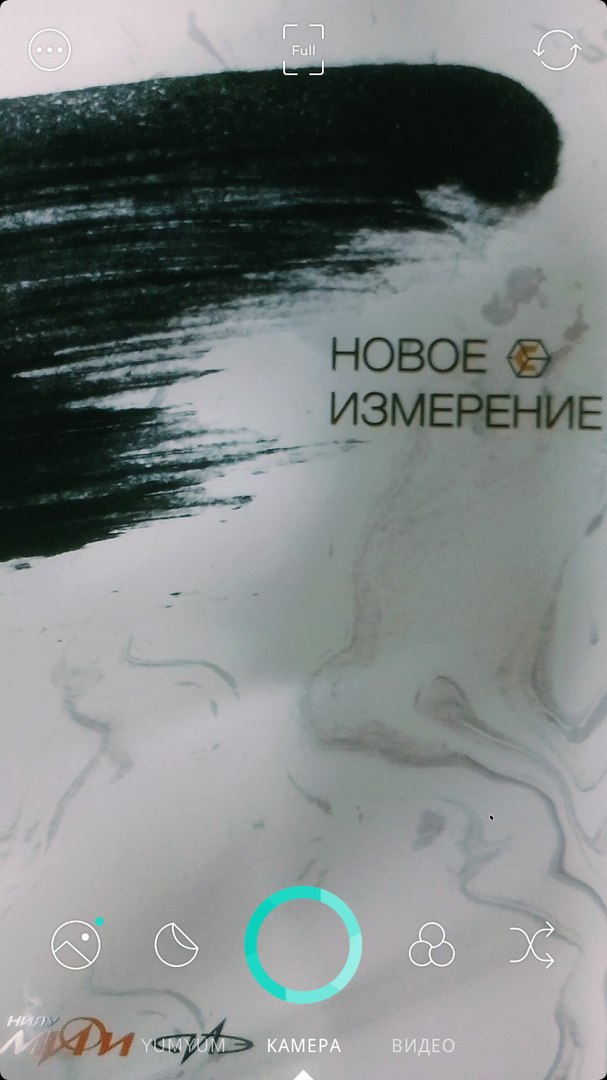
\includegraphics[width=0.3\linewidth]{pics/candyCam}
	\caption{Candy Camera, окно с камерой}
	\label{fig:candyCam}
\end{figure}

\begin{figure}[H]
	\centering
	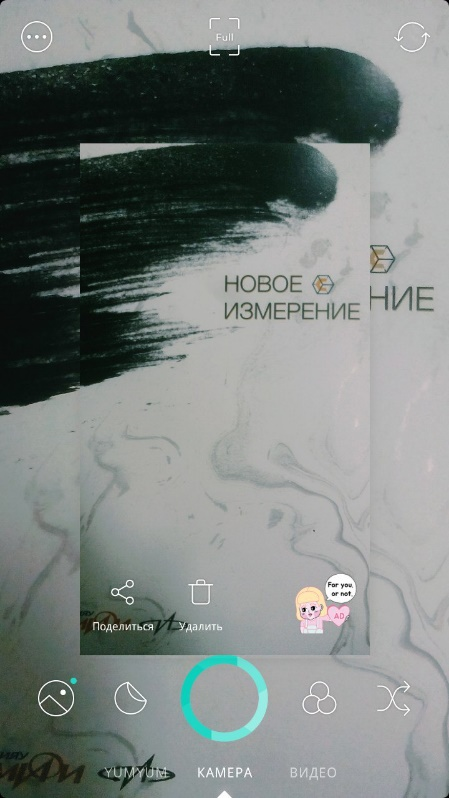
\includegraphics[width=0.3\linewidth]{pics/candyGal}
	\caption{Candy Camera, окно с просмотром фото}
	\label{fig:candyGal}
\end{figure}

\begin{figure}[H]
	\centering
	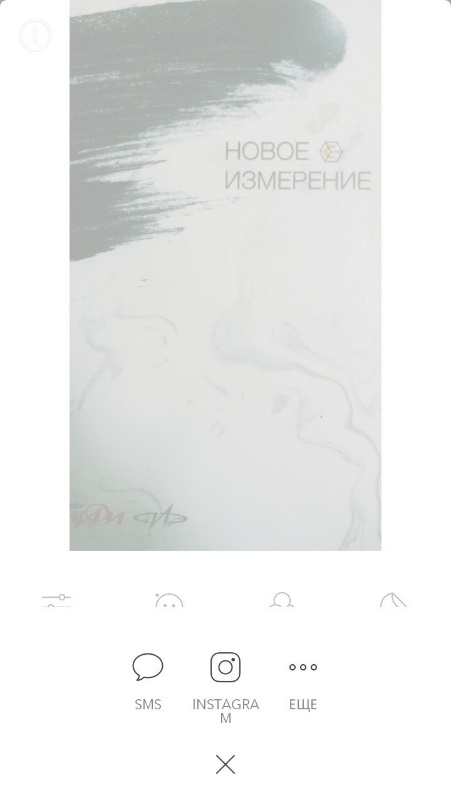
\includegraphics[width=0.3\linewidth]{pics/candyPod}
	\caption{Candy Camera, окно выбора с кем поделиться изображением}
	\label{fig:candyPod}
\end{figure}

\subsection{Pixlr}
Проанализировав пользовательский интерфейс приложения Pixlr (рисунок~\ref{fig:pixlrMenu}), основное различие с предыдущими приложениями это наличие главного меню, которое открывается при запуске программы. В меню можно выбрать дальнейшее действие, открыть камеру и сделать фотографию или открыть галерею и выбрать картинку из имеющихся изображений. Из режима камеры нельзя перейти в галерею (рисунок~\ref{fig:pixlrCam}). Имеются кнопки с фильтрами, которые применяются сразу. Сделав фотографию, мы оцениваем ее и решаем сделать новое фото или продолжить редактировать. Галерея открывается с помощью стандартного просмотрщика галереи этого телефона. Применив фильтр, Pixlr предлагает разместить фото в разных социальных сетях, сохранить изображение или выбрать дополнительные действия с картинкой (рисунок~\ref{fig:pixlrPod}). При сохранении можно выбрать разрешение, формат JPEG или PNG и качество изображения, после сохранения остается возможность поделиться этой фотографией в социальных сетях.

\begin{figure}[H]
	\centering
	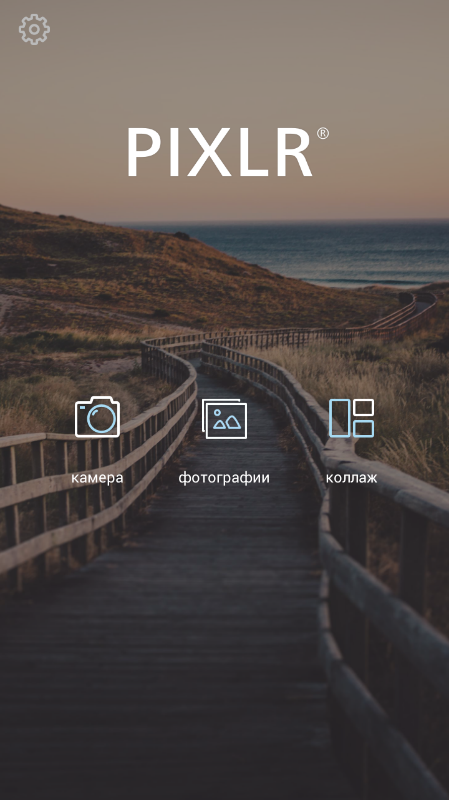
\includegraphics[width=0.3\linewidth]{pics/pixlrMenu}
	\caption{Pixlr, главное меню}
	\label{fig:pixlrMenu}
\end{figure}

\begin{figure}[H]
	\centering
	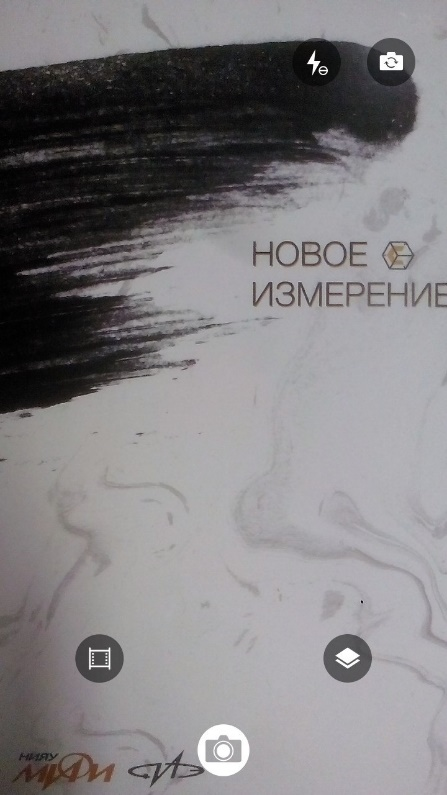
\includegraphics[width=0.3\linewidth]{pics/pixlrCam}
	\caption{Pixlr, окно с камерой}
	\label{fig:pixlrCam}
\end{figure}

\begin{figure}[H]
	\centering
	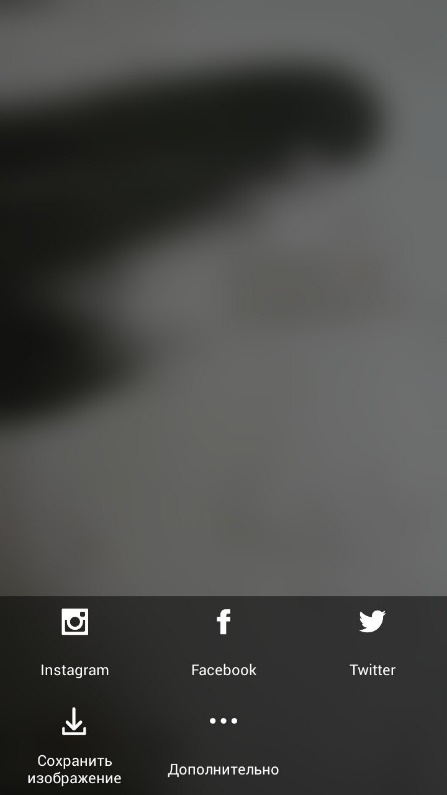
\includegraphics[width=0.3\linewidth]{pics/pixlrPod}
	\caption{Pixlr, окно выбора с кем поделиться изображением}
	\label{fig:pixlrPod}
\end{figure}

\subsection{Анализ интерфейса}
Сравнив данные приложения, увидели общие черты, в режиме камеры имеются кнопки переключения режима фотовспышки и переключение между основной и фронтальной камерами. Есть возможность выбора соотношений, пропорций фотографии. Везде есть возможность поделиться фотографией в Instagram.

У Pixlr есть отличительная черта, это наличие главного меню и отсутствие собственного пользовательского интерфейса галереи. У Prisma, интерфейс галереи реализован лучше чем у Candy Camera. У Pixlr и Candy Camera есть удобная возможность просматривать фильтр в живую, еще не сделав фотографии. В режиме камеры у Pixlr и Prisma, кнопки расположены и выглядят более удобно чем у Candy Camera. Окно выбора действия с отредактированным изображением (сохранить или поделиться фотографией в социальных сетях) у Pixlr реализовано лучше.

Считаю, что необходимый набор функций программы должен включать: выбор фотографии из стандартной галереи, режим камеры, обработка изображения, просмотр результата, возможность сохранить, поделиться фотографией в социальных сетях и дополнительные возможности передачи картинки.

Необходимый набор элементов пользовательского интерфейса камеры должен включать: переключение режимов фотовспышки, переключение главной и фронтальной камеры, кнопку настроек, переход к выбору фотографии из галереи.

Мы планируем сделать приложение следующим образом, при включении откроется камера (рисунок~\ref{fig:cam}), сделав фотографию пользователю предстоит оценить получившуюся фотографию и если нравится, то перейти к редактированию изображения, иначе сделать новое фото (рисунок~\ref{fig:foto}). Сделав удовлетворяющую фотографию или выбрав нужную из галереи, происходит обработка изображения, и пользователь может просмотреть получившуюся картинку. Тут же есть возможность вернуться к камере, обрезать или продолжить. Выбрав продолжить, появляется окно с выбором дальнейших действий с данной фотографией, запостить фото в социальных сетях на выбор, сохранить изображение в пользовательском качестве или дополнительные способы передачи картинки (рисунок~\ref{fig:pod}).

\begin{figure}[H]
	\centering
	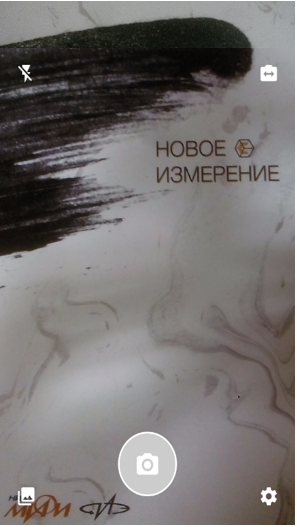
\includegraphics[width=0.3\linewidth]{pics/cam}
	\caption{Окно с камерой}
	\label{fig:cam}
\end{figure}

\begin{figure}[H]
	\centering
	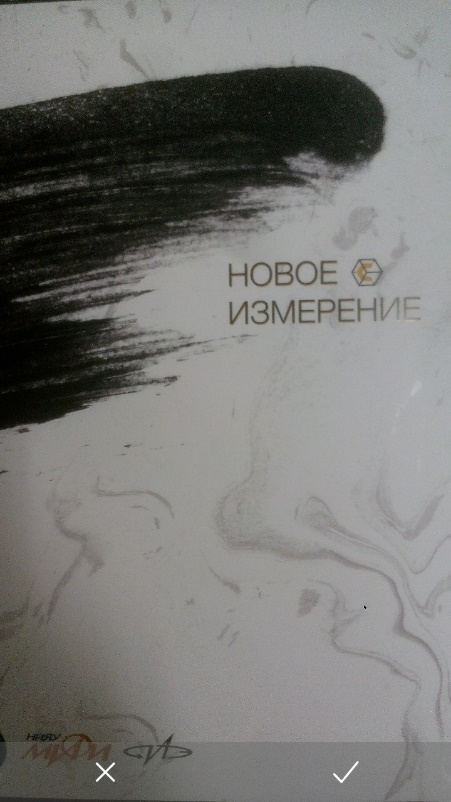
\includegraphics[width=0.3\linewidth]{pics/foto}
	\caption{Окно с просмотром фото}
	\label{fig:foto}
\end{figure}

\begin{figure}[H]
	\centering
	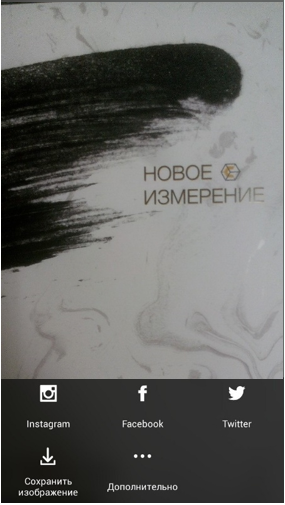
\includegraphics[width=0.3\linewidth]{pics/pod}
	\caption{Окно выбора с кем поделиться изображением}
	\label{fig:pod}
\end{figure}

При создании пользовательского интерфейса приложения были проанализированы современные, с аналогичным функционалом мобильные приложения в целом. Был сделан акцент на необходимости создания современного, функционального и не перегруженного пользовательского интерфейса. В результате проведенного анализа был создан пользовательский интерфейс мобильного приложения для преобразования 2D фотографий в 3D вид.



// Дубль

\section{Анализ существующих продуктов со схожим функционалом}
В ходе подготовки к процессу разработки приложения был проведен анализ магазина мобильных приложений (Google Play) для проверки на наличие аналогичных разработок или разработок схожей тематики.

По результатам анализа оказалось, что такой реализации преобразования фотографий в 3D нет. Однако в этой категории есть ряд похожих разработок, направленных на оживление «плоских» снимков. 

\subsection{Make It 3d Free}

Приложение, позволяющее создать красно-синий анаглиф либо на основе снимка из фотогалереи смартфона, либо сделав снимок прямо из приложения. Стоит заметить, что анаглиф создается на основе двух снимков:  левого и правого, - что само по себе является естественным способом создание объемного изображения, а значит должно гарантировать получение качественного 3D-изображения. После прикрепления двух изображений доступны возможности изменения стереоэффекта: смещение или поворот одного из изображений по или против часовой стрелки. Есть возможность сохранения результата в виде широкого изображения с разделением зон на правый и левый глаз, что может пригодиться для просмотра снимка в устройстве виртуальной реальности (например, в кардборде). По завершении работы, фото экспортируется в галерею и открывается стандартном просмотрщике изображений девайса. (рисунок ~\ref{fig:MakeIt})

\begin{figure}[H]
	\centering
	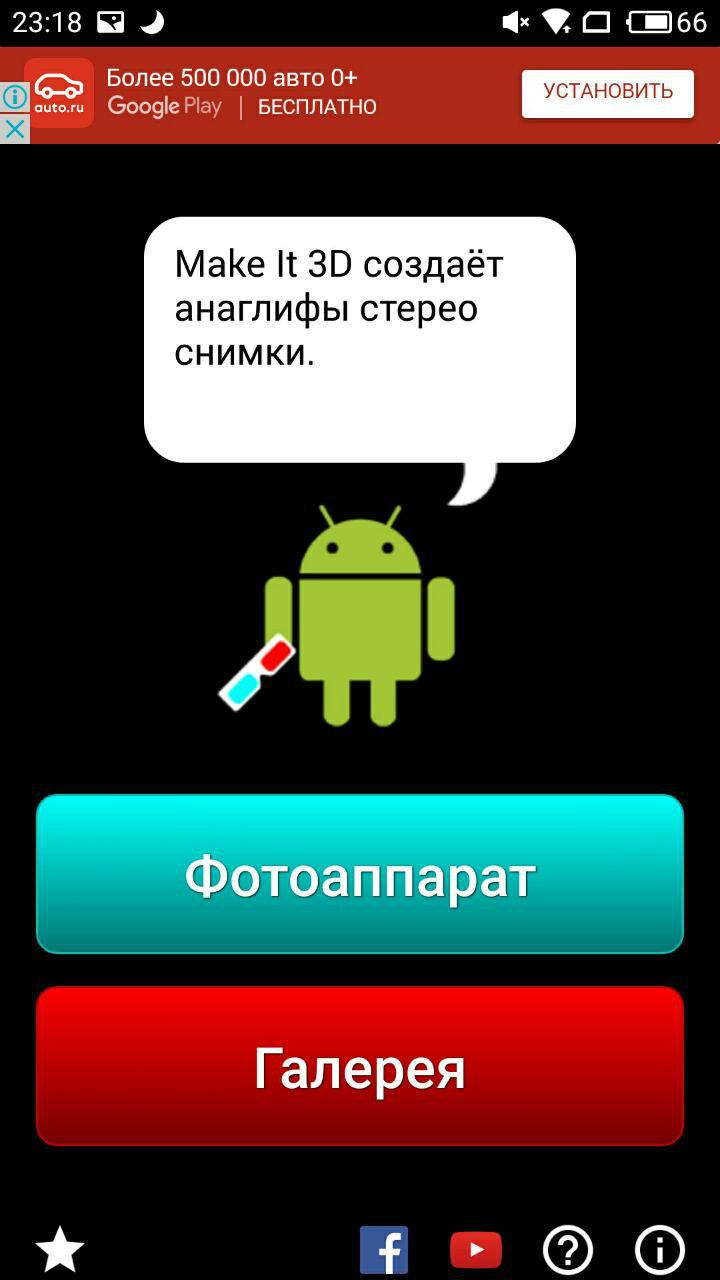
\includegraphics[width=0.45\linewidth]{pics/MakeIt1}
	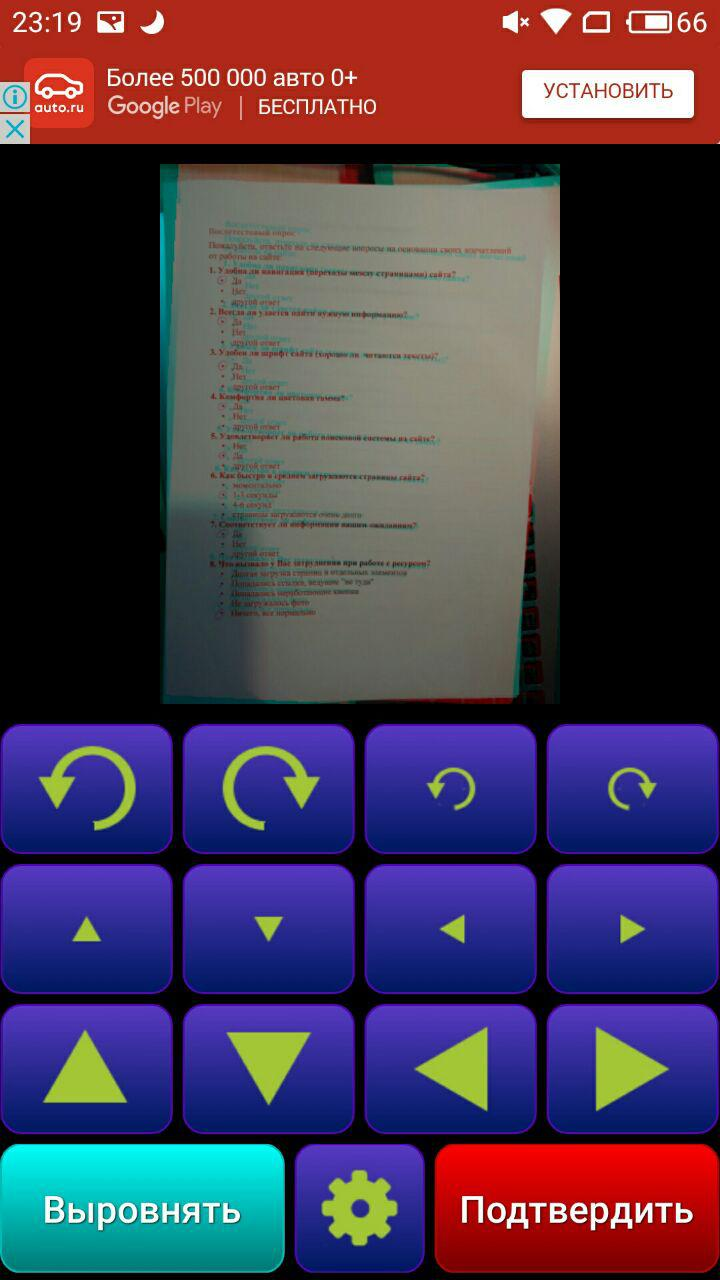
\includegraphics[width=0.45\linewidth]{pics/MakeIt2}
	\caption{MakeIt}
	\label{fig:MakeIt}
\end{figure}

\subsection{3D Effect}

Приложение, создающее анаглиф из одного изображения. Доступна возможность настройки степени смещение и выбор одного из трех вариантов смещения:  по горизонтали, по вертикали, по диагонали. Так предоставлена возможность выбора цвета стереоэффекта, например: красно-голубой, сине-желтый, зелёно-розовый. Изображение сохраняется в фотогалерею смартфона и выводит варианты «шэринга». (рисунок ~\ref{fig:3dEffect})

\begin{figure}[H]
	\centering
	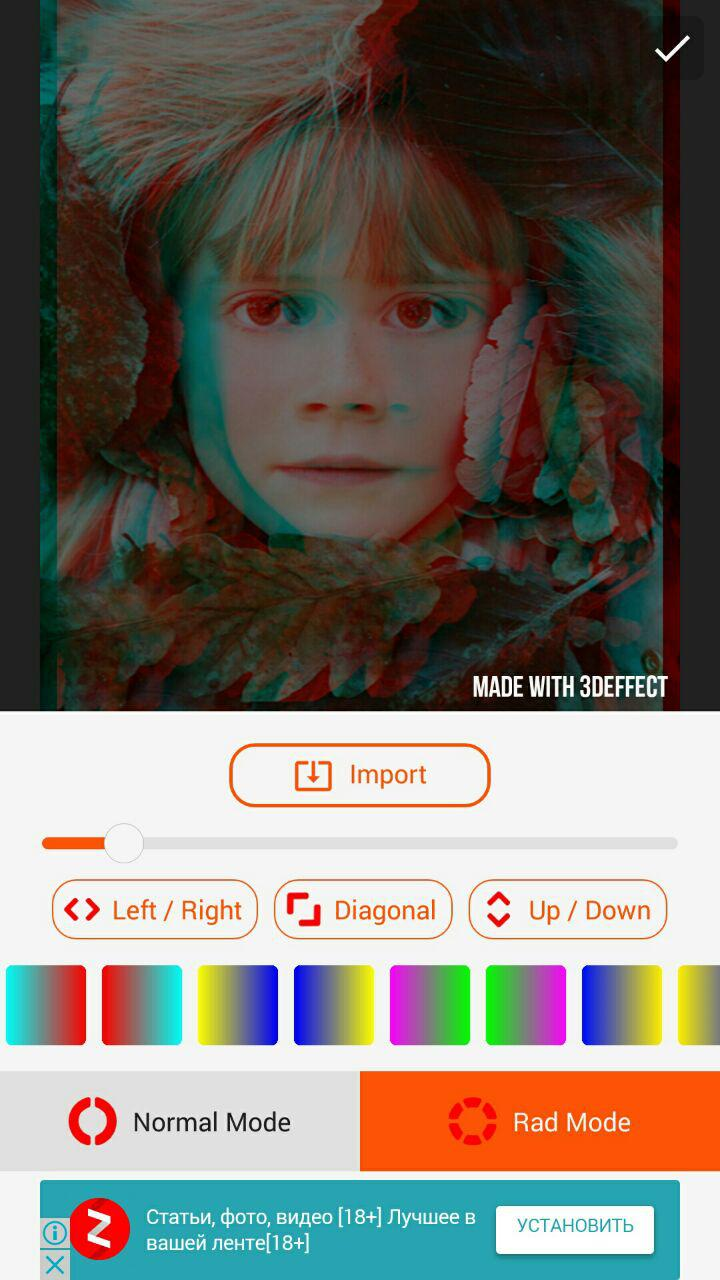
\includegraphics[width=0.45\linewidth]{pics/3dEffect1}
	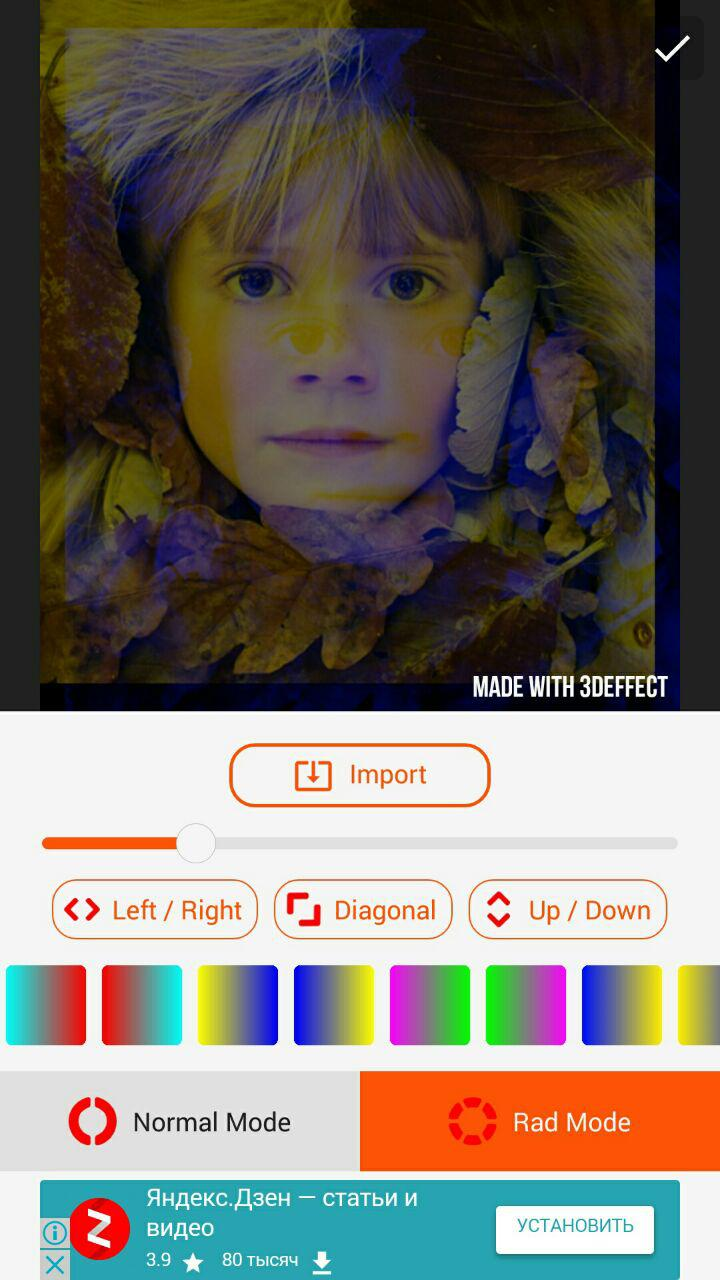
\includegraphics[width=0.45\linewidth]{pics/3dEffect2}
	\caption{3dEffect}
	\label{fig:3dEffect}
\end{figure}

\subsection{Motion Photo}

Инструмент, предоставляемый производителями смартфонов. Впервые появился в iOS 9 в 2015 году под названием Live Photos, а позже аналоги появились в Android-смартфонах, линейке Galaxy от Samsung, начиная с модели S7, а также в Google Pixel 2. Решение в корне отличается от варианта с созданием анаглифа, однако предоставляет возможность оживить фотографию, что так же является и результатом работы нашей разработки. Принцип работы заключается в постоянном сохранении в оперативную память устройства 1-3 секунд изображения с камеры, до момента нажатия на кнопку спуска затвора, после чего сохраняется еще один видеофрагмент. Таким образом, при просмотре обычного фото в галерее смартфона, появляется возможность увидеть живой момент съемки.

\subsection{Fyuse}

Fyuse совмещает в себе возможность создания пространственной фотографии и платформу для общения. По ходу использования приложение фокусируется на объекте, а затем при помощи графических подсказок на экране предлагает обойти объект камерой по орбите. Полученный результат представляет собой снимок, позволяющий перемещать камеру вида по орбите вокруг изображенного предмета при помощи свайпов или гироскопа смартфона. Фотографию можно сохранить или опубликовать прямо во Fyuse, являющейся так же и социальной сетью. (рисунок ~\ref{fig:Fyuse})

\begin{figure}[H]
	\centering
	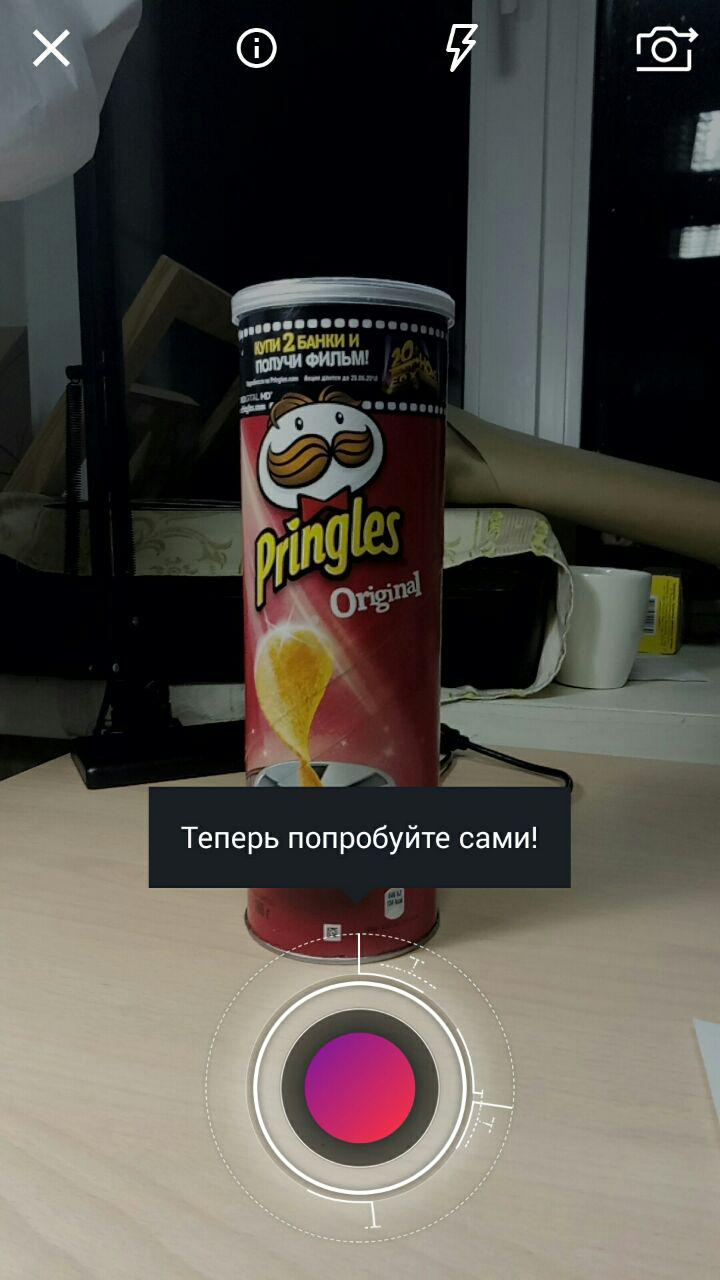
\includegraphics[width=0.45\linewidth]{pics/Fyuse1}
	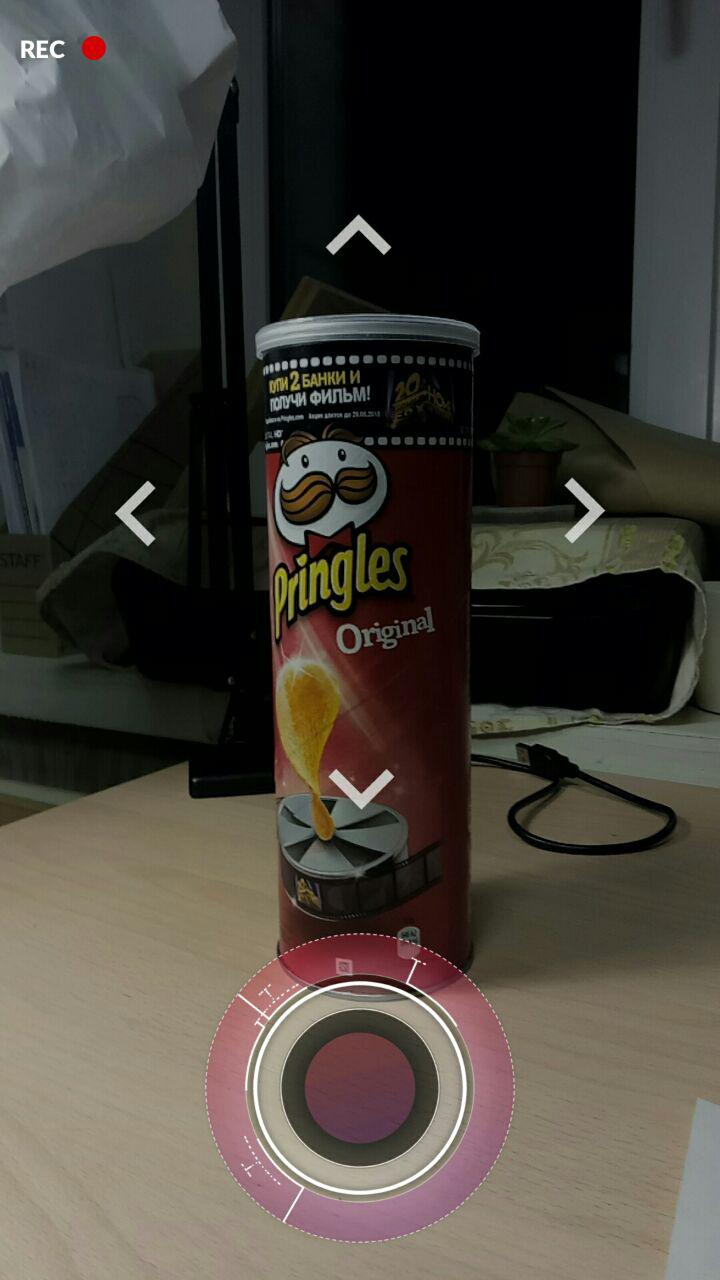
\includegraphics[width=0.45\linewidth]{pics/Fyuse2}
	\caption{Fyuse}
	\label{fig:Fyuse}
\end{figure}

\subsection{Вывод}
По результатам анализа существующих аналогов можно сделать вывод, что разработчики предлагают абсолютно разные способы оживления снимков. Для некоторых требуются определенный манипуляции еще при съемке, некоторые могут работать с готовыми фотографиями. Каждое решение по-своему уникально и интересно. Мы же предлагаем еще одно решение, особенностью которого является «оживление» уже готового снимка.


\section{Разработка пользовательского интерфейса мобильного приложения (UI/UX)}

Одна из важнейших задач в ходе создания мобильного приложения, преобразовывающего 2D снимки в объемные (3D) - разработка удобного и интуитивно-понятного пользовательского интерфейса. UI/UX (user Interface, user experience) составляющая, она же пользовательский интерфейс и пользовательский опыт, является более чем просто значимым элементом современного мобильного приложения. Удобство расположения элементов управления и приятное визуальное оформление напрямую влияют на настроение пользователя при использовании продукты. Именно некачественный UI/UX-дизайн отпугивает людей от использования многих приложений в пользу их более достойных альтернатив.

\subsection{Анализ интерфейсов смежных приложений}

Для использования качестве референсов были подобраны приложения, принадлежащие широкому понятию «Приложения для работы с фото», так как узкоспециализированные решения не представляют интерфейса должного качества и удобства.

В список приложений для анализа попали такие приложения, как:  Prisma, Vinci, Snapster и Pixlr.

В первую очередь, целью сравнения являлся анализ особенностей пользовательского интерфейса этих приложений. Это обусловлено тем, что предполагаемая схема  взаимодействия пользователя с разрабатываемым приложением во много схожа с таковой в этих приложениях, за исключением некоторых их особенностей. Важные элементы для сравнения  - сценарий создания снимка с использованием фотокамеры смартфона и выбор снимка из галереи для дальнейшей отправки фотографии на обработку алгоритмом, преобразующим ее в 3D фотографию.

\subsubsection{Prisma}

Проанализировав пользовательский интерфейс первого приложения, Prisma (рисунок~\ref{fig:prisma}), можно заметить не очень удобное расположение элементов. Так, кнопка настроек, далеко не самая востребованная на фоне остальных, расположена в правом нижнем углу, куда доступ наиболее прост в условиях больших размеров современных смартфонов. В том время как кнопка смена камеры расположена в правом верхнем углу, куда доступ затруднительнее. Стоит отметить и факт смещения нижних иконок в углу экрана, что далеко не положительном образом сказывается на опыте использования приложения.

Также Prisma, в связи со своими социальными особенностями функционала, имеет навигационный бар в верхней части экрана, представленный фиксированными вкладками (fixed tabs), оформленным в соответствии с гайдлайнами material-дизайна (Material Design Guidelines), разработанными Google. В целом приложение лишь частично следует гайдлайнам от Google, что заметно на примере применения material-иконок и одновременно неверном использовании фаба (float action button).

Экран шейринга фотографии выполнен по примеру Instagram, с подобным размещением элементов и учетом особенностей Prisma.

\begin{figure}[H]
	\centering
	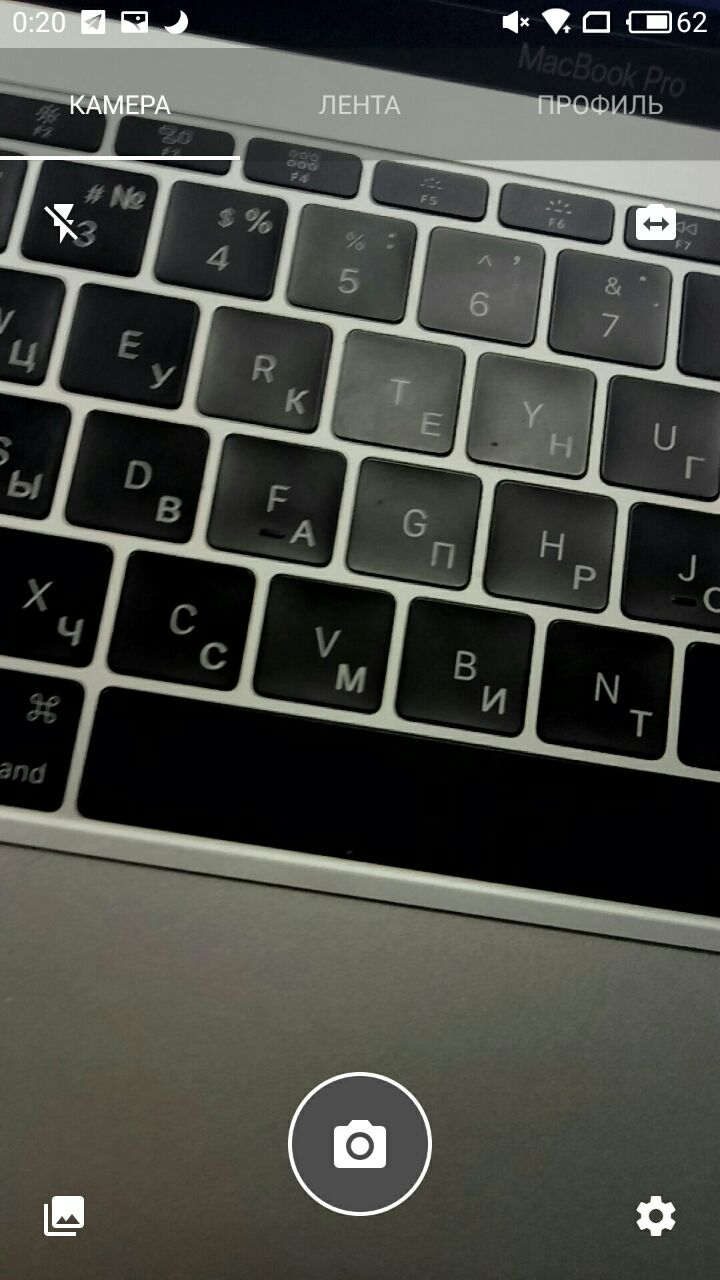
\includegraphics[width=0.45\linewidth]{pics/prisma1}
	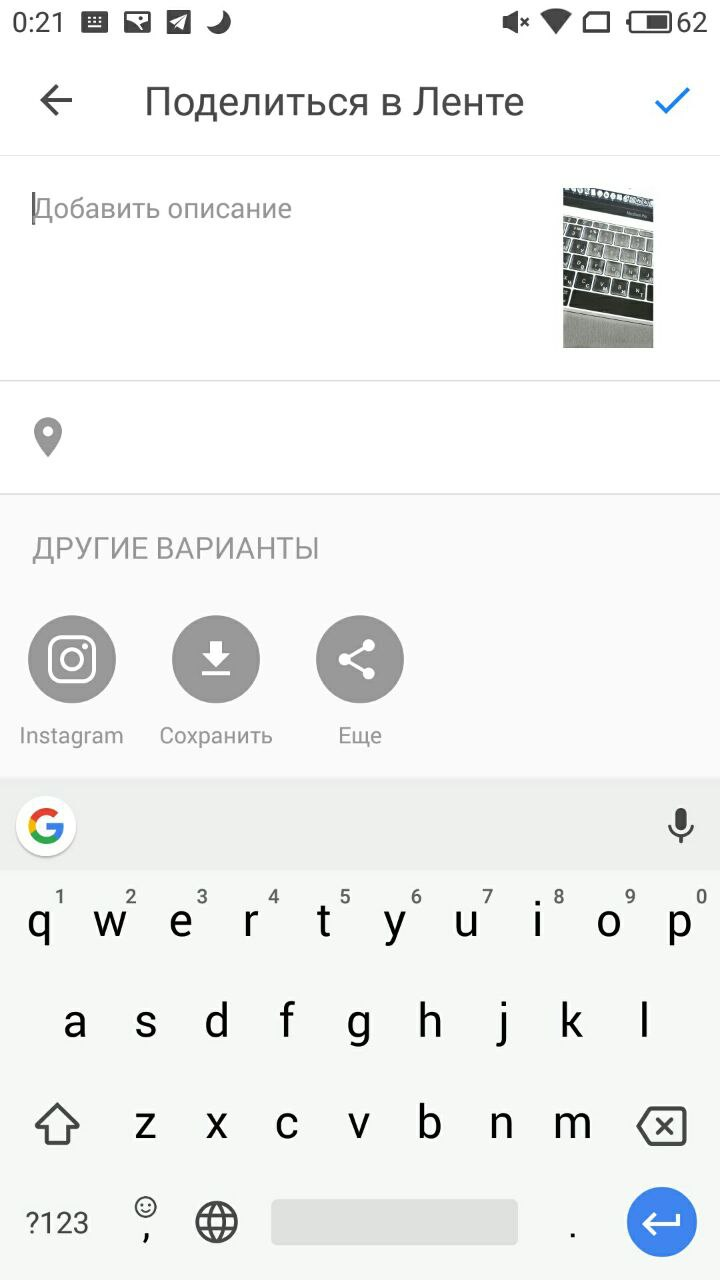
\includegraphics[width=0.45\linewidth]{pics/prisma2}
	\caption{Prisma}
	\label{fig:prisma}
\end{figure}

\subsubsection{Vinci}

Интерфейс Vinci (рисунок~\ref{fig:vinci}) выглядит более удачным, на фоне Prisma, и, забегая вперед, на фоне остальных выбранных приложений также, за исключением  Snapster. В нижней части удачно разместилась  выдвигающаяся панель с последними снимками, выше кнопка спуска затвора, включения вспышки и смены камеры. В верхнем углу разместилась иконка настроек. Такое разделение экрана обусловлено популярным соотношением сторон для снимков 4:3.

Плашка шейринга, появляющаяся в нижней части экрана, также весьма удобна для использования.

\begin{figure}[H]
	\centering
	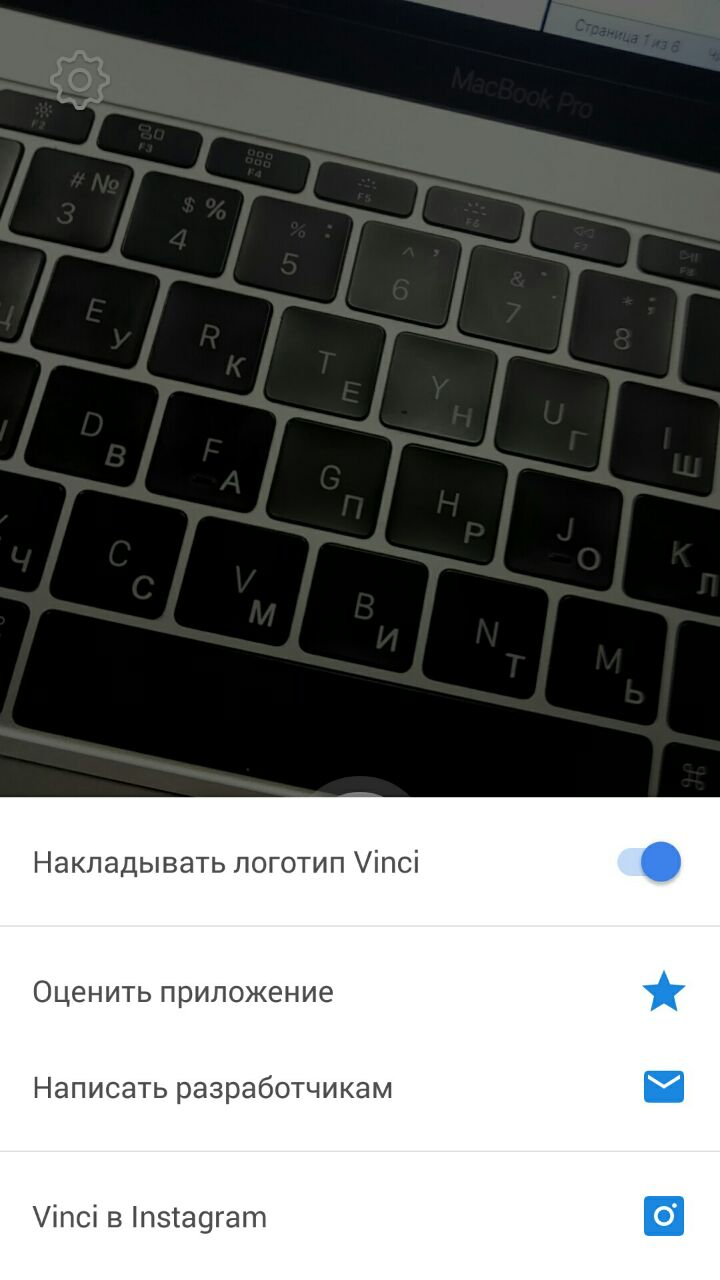
\includegraphics[width=0.3\linewidth]{pics/vinci1}
	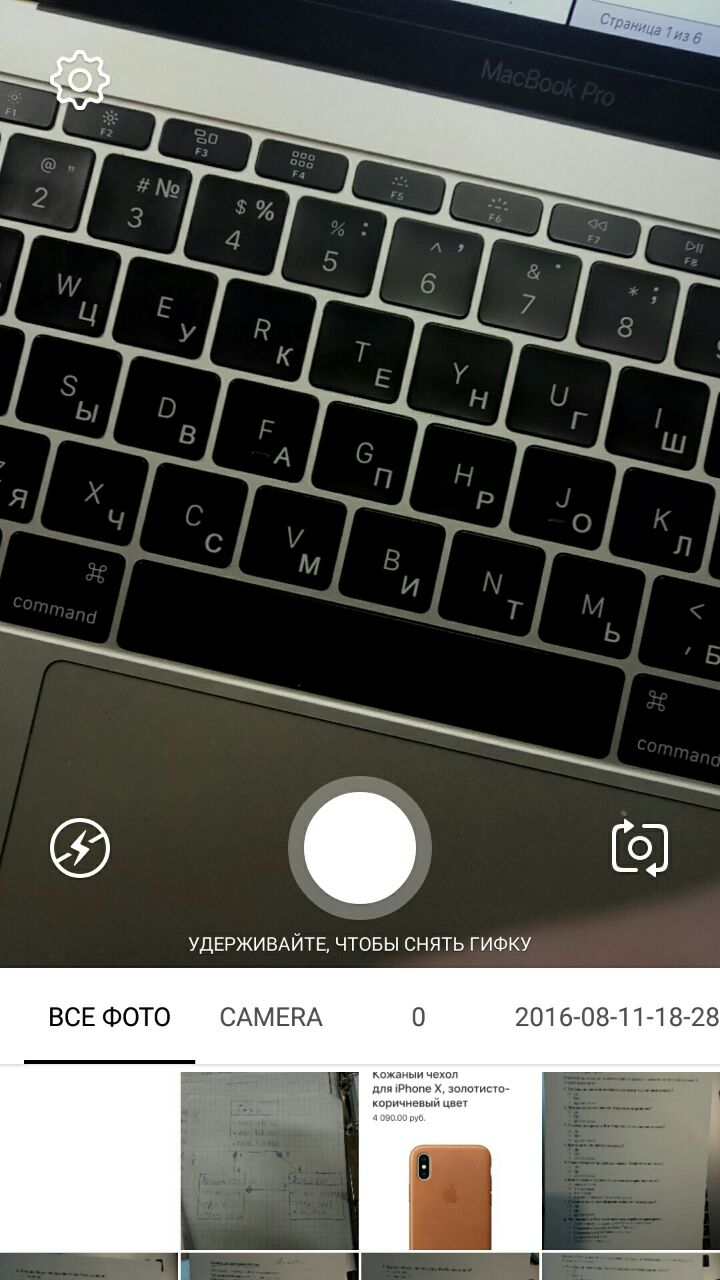
\includegraphics[width=0.3\linewidth]{pics/vinci2}
	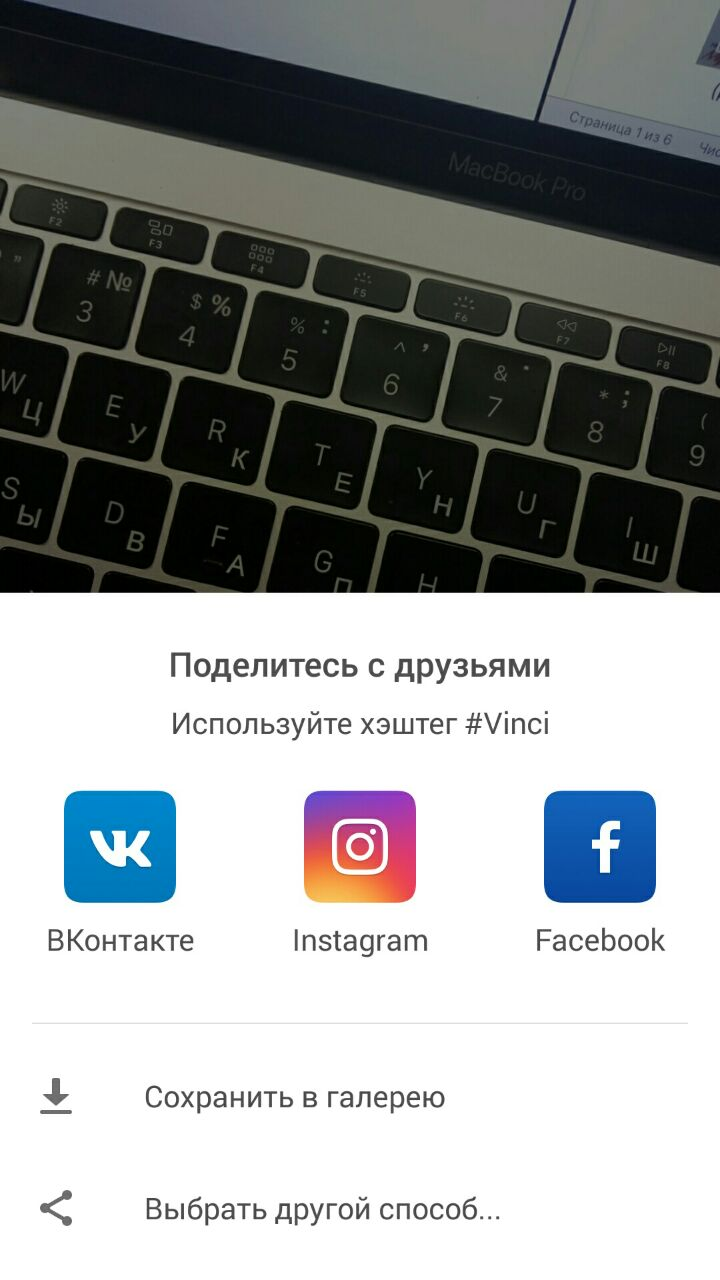
\includegraphics[width=0.3\linewidth]{pics/vinci3}
	\caption{Vinci}
	\label{fig:vinci}
\end{figure}

\subsubsection{Pixlr}

Особенностью интерфейса Pixlr (рисунок~\ref{fig:pixlr}),  в отличие от подобранных примеров, я является присутствие стартового экрана, который, однако, несколько замедляет взаимодействие с приложением. Кнопки управление на экране камеры визуально неприятны и имеют непривычное соотношение размеров.

\begin{figure}[H]
	\centering
	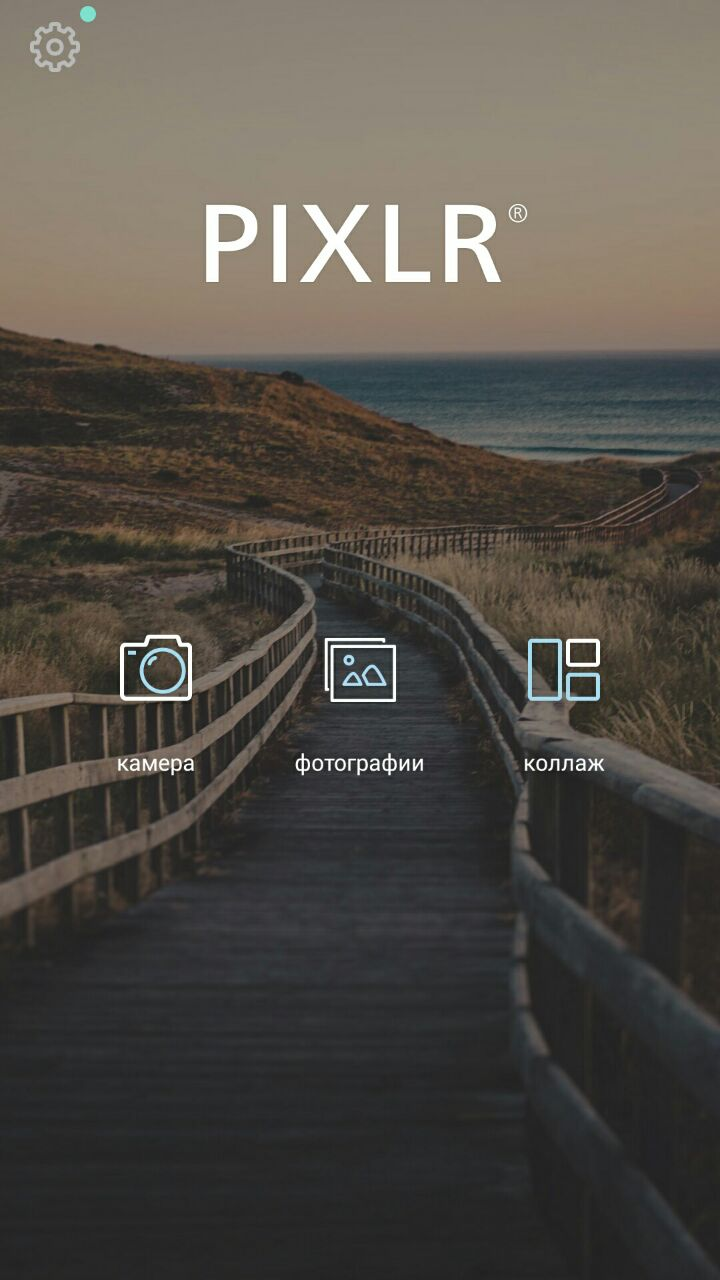
\includegraphics[width=0.45\linewidth]{pics/pixlr1}
	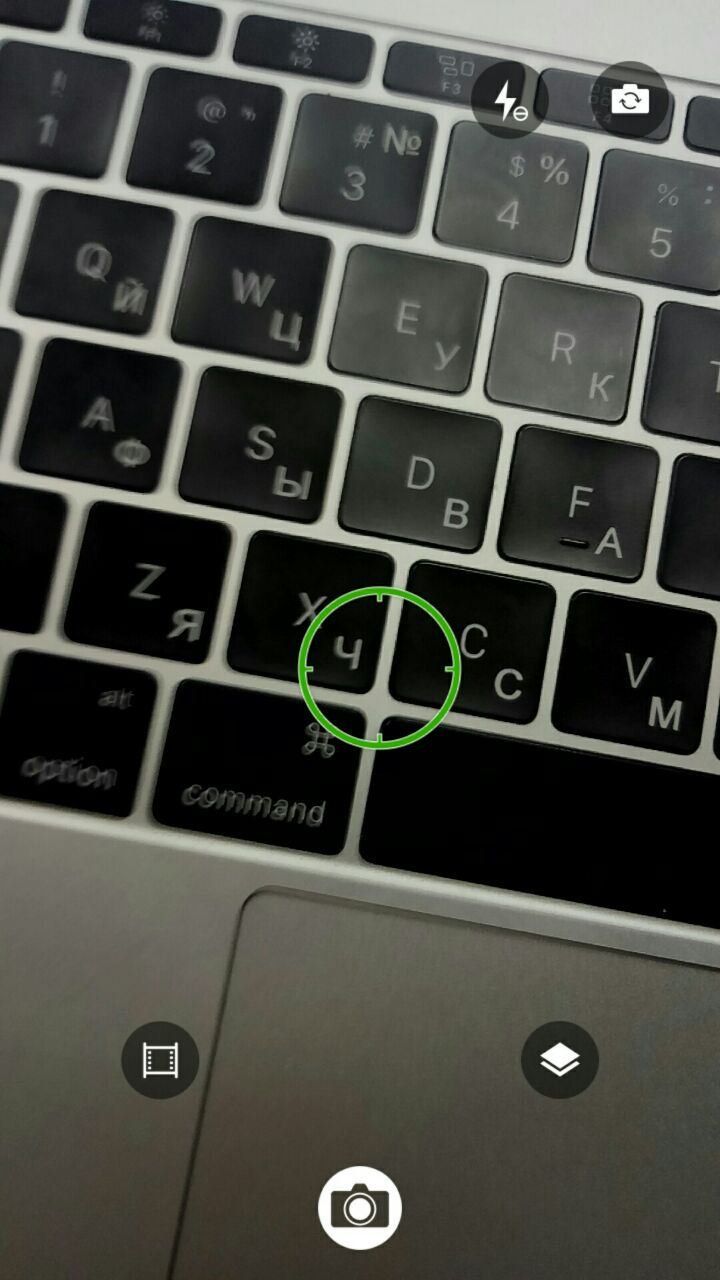
\includegraphics[width=0.45\linewidth]{pics/pixlr2}
	\caption{Pixlr}
	\label{fig:pixlr}
\end{figure}

\subsubsection{Snapster}

Как уже было сказано, Vinci и Snapster (рисунок~\ref{fig:snapster}) имеют примерно одинаковый уровень юзабилити, что объясняется одним и тем же авторством. В нижней части экрана размещен блок с последними снимками, но уже другим способ навигации - горизонтальной прокруткой (скроллом). Разработчик решил не внедрять кнопку настроек, нашлось место для полезно кнопки активации сетки. В целом, приложение Snapster, являясь экспериментальным проектом социальной сети VK, претерпело за время своего существования довольно сильные изменения. Если в первоначальном виде приложение дублировало основной функционал модуля «Фотографии» из социальной сети VK и расширяло его возможности, то сейчас, не сыскав популярности, было урезано до простенького фоторедактора.

\begin{figure}[H]
	\centering
	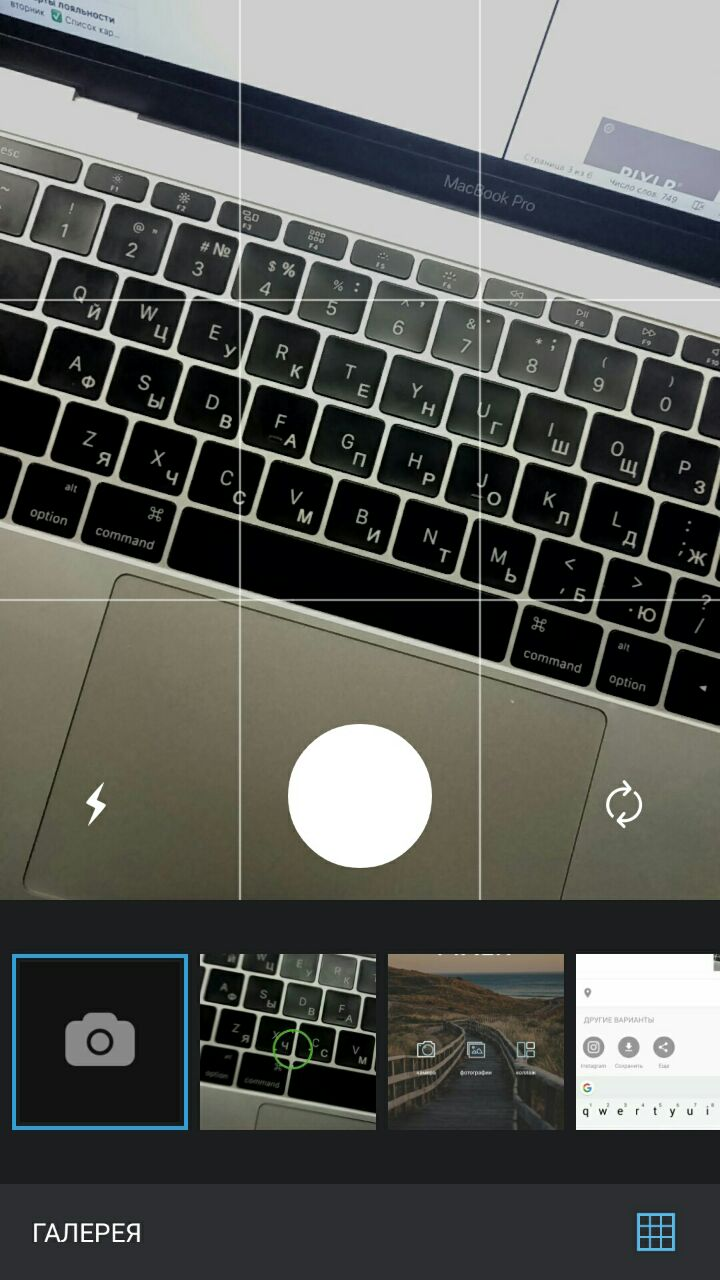
\includegraphics[width=0.45\linewidth]{pics/snapster1}
	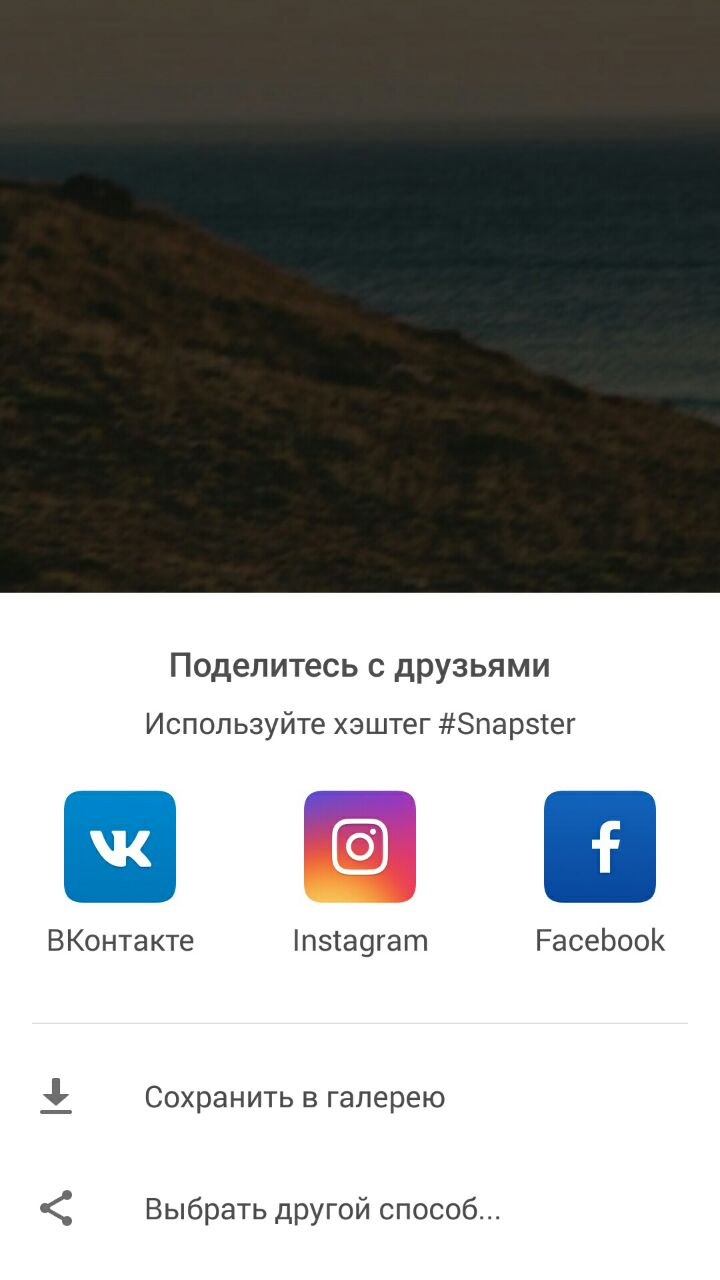
\includegraphics[width=0.45\linewidth]{pics/snapster2}
	\caption{Snapster}
	\label{fig:snapster}
\end{figure}

\subsection{Разработка пользовательского интерфейса мобильного приложения (UI/UX)}

Интерфейс Android-смартфона мобильного приложения для преобразования 2D фотографии в 3D вид выполнен в соответствии с гайдлайнами Material Design. Отступы, иконки и используемые шрифты полностью соответствуют руководству от Google~\cite{google}. 

Расположение элементов управление выполнено с учетом лучших особенностей приложений-аналогов.

На главный экран камеры (рисунок~\ref{fig:Artboard}) выведены следующие функции:

\begin{itemize}
	\item Спуск затвора;
	\item Выбор фото из галереи;
	\item Смена камеры;
	\item Управление вспышкой;
	\item Переход к настройкам и справке.
\end{itemize}

\begin{figure}[H]
	\centering
	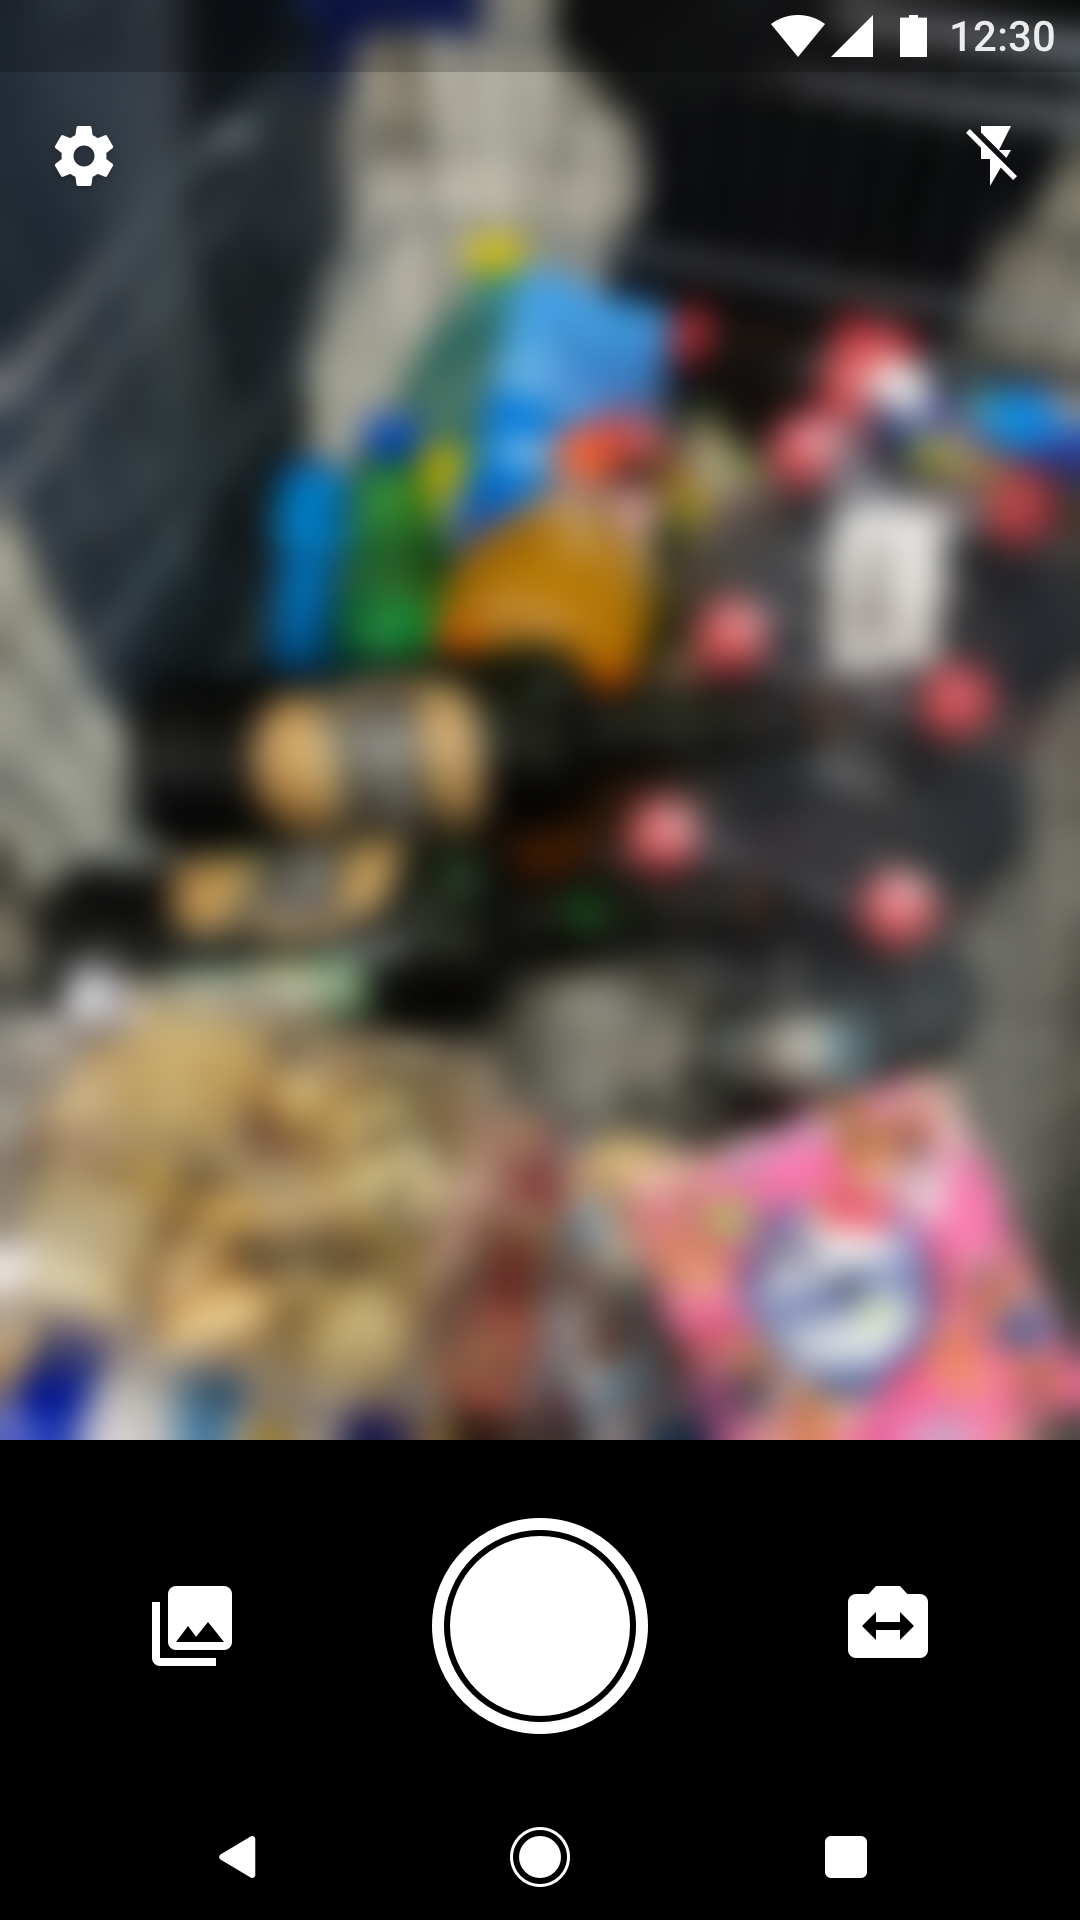
\includegraphics[width=0.6\linewidth]{pics/Artboard}
	\caption{Окно с камерой}
	\label{fig:Artboard}
\end{figure}

На экране с обработанной фотографией по нажатии кнопки «Далее» появляется bottom sheet (рисунок~\ref{fig:Artboard2}), включающий в себя быстрые функции шеринга и сохранения полученного фото в галерею.

\begin{figure}[H]
	\centering
	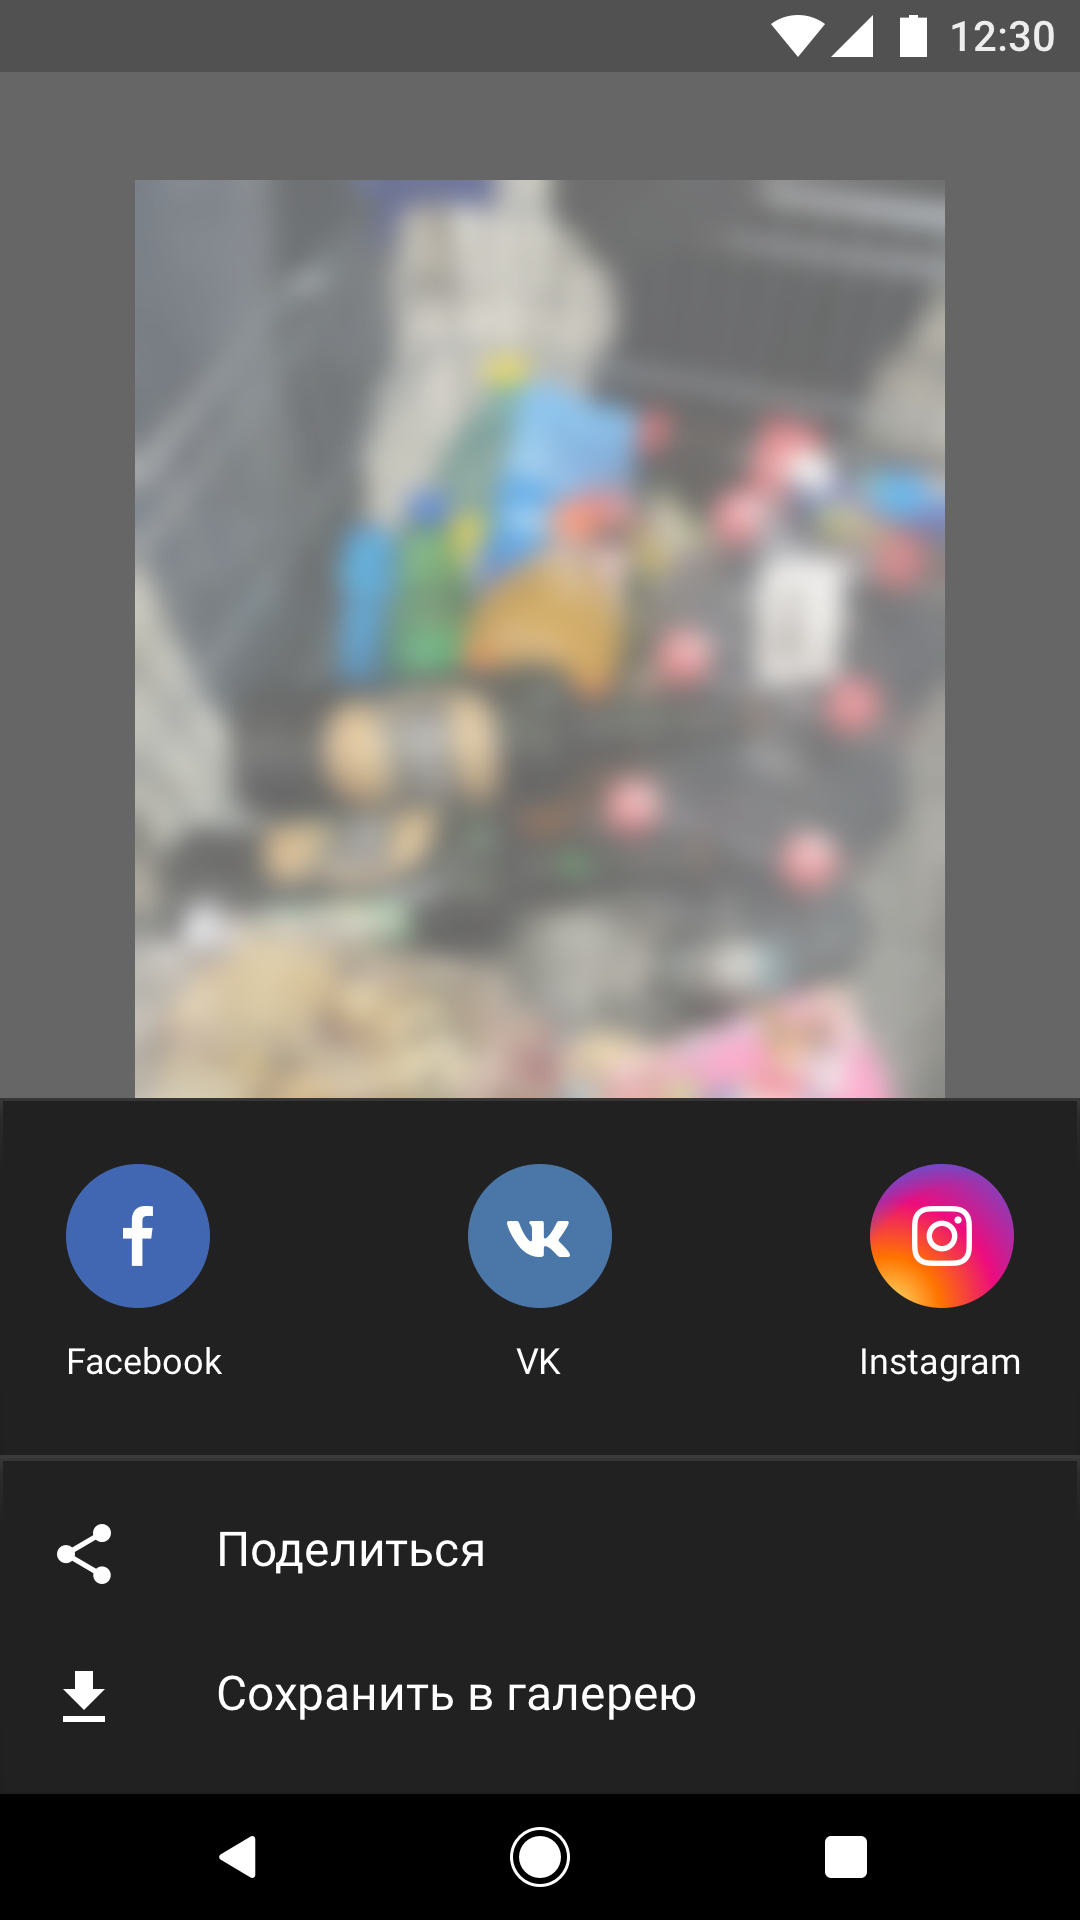
\includegraphics[width=0.6\linewidth]{pics/Artboard2}
	\caption{Окно с просмотром фото}
	\label{fig:Artboard2}
\end{figure}

При создании пользовательского интерфейса приложения были проанализированы современные, с аналогичным функционалом мобильные приложения в целом. Был сделан акцент на необходимости создания современного, функционального и не перегруженного пользовательского интерфейса. В результате проведенного анализа был создан пользовательский интерфейс мобильного приложения для преобразования 2D фотографий в 3D вид.



% НИР2

\section{Описание предметной области}
В ходе выполнения проекта, главным образом, решается задача преобразования двумерных изображений в трехмерные(GIF) на мобильных устройствах.

В последние годы заметное место в области преобразования и фильтрации изображений занимает задача преобразования двумерных изображений в трехмерные. На сегодняшний день в мире для этого разработаны различные методики, которые позволяют автоматически создавать так называемые «карты глубины» для двумерных изображений, основываясь на свойствах этого изображение и на некоторых предположениях о характере сцены. 

\subsection{Android Studio}
Android Studio - полностью укомплектованная платформа для разработки и тестирования приложений под операционную систему Android. Разработчики этой оболочки (компания Google) внедрили весь необходимый инструментарий для удобного и качественного проектирования новых приложений и доработки существующих. Программа включает в себя такие компоненты как Android SDK, все версии операционки Android, эмулятор для запуска приложений, элементы тестирования и отладки программ.

Создавая новый проект, будет доступна полная структура приложения со всеми файлами, что позволяет более четко и продуманно организовать сам процесс разработки. Очень удобно реализован показ вносимых изменений и дополнений - визуально в реальном времени происходят преобразования в зависимости от заданных действий. Что немаловажно, программа позволяет делать разработку приложений для всех версий ОС Andriod и для различных устройств - можно предварительно оценить внешний вид программы, например, под планшет или смартфон.

Среда Android Studio предназначена как для небольших команд разработчиков мобильных приложений (даже в количестве одного человека), или же крупных международных организаций с GIT или другими подобными системами управления версиями. Опытные разработчики смогут выбрать инструменты, которые больше подходят для масштабных проектов. Решения для Android разрабатываются в Android Studio с использованием Java или C++. В основе рабочего процесса Android Studio заложен концепт непрерывной интеграции, позволяющий сразу же обнаруживать имеющиеся проблемы. Продолжительная проверка кода обеспечивает возможность эффективной обратной связи с разработчиками. Такая опция позволяет быстрее опубликовать версию мобильного приложения в Google Play App Store. В Android Studio есть удобная маркировка кода, которая позволит без труда ориентироваться в больших проектах. Кроме того, отдельные компоненты можно изменять простым перетаскиванием в другое нужное место, что значительно упрощает редактирование.

\subsection{Java}
Преимущества языка Java
\begin{itemize}
	\item Одно из основных преимуществ языка Java — независимость от платформы, на которой выполняются программы: один и тот же код можно запускать под управлением операционных систем Windows, Solaris, Linux, Machintosh и др. 
	Это действительно необходимо, когда программы загружаются через Интернет для последующего выполнения под управлением разных операционных систем.
	\item Другое преимущество заключается в том, что синтаксис языка Java похож на синтаксис языка C++, и программистам, знающим языки С и C++, его изучение не составляет труда.
	\item Кроме того, Java — полностью объектно-ориентированный язык, даже в большей степени, чем C++. Все сущности в языке Java являются объектами, за исключением немногих основных типов (primitive types), например чисел.
	\item Исключена возможность явного выделения и освобождения памяти.	Память в языке Java освобождается автоматически с помощью механизма сборки мусора. Программист гарантирован от ошибок, связанных с неправильным использованием памяти.
	\item Безопасный: методы проверки подлинности основаны на шифровании с открытым ключом.
	\item Динамический: программирование на Java считается более динамичным, чем на C или C++, так как он предназначен для адаптации к меняющимся условиям. Программы могут выполнять обширное количество во время обработки информации, которая может быть использована для проверки и разрешения доступа к объектам на время выполнения.
\end{itemize}

\subsection{Выбор архитектуры мобильного приложения}
В ходе выполнения работы были рассмотрены различные варианты для создания мобильных приложений, предназначенных для преобразования 2D изображений в 3D вид. При этом рассмотрении учитывалось, что результирующие мобильные приложения должны создаваться под операционные системы Android, а также то, что один из основных результатов работы приложения с точки зрения конечного пользователя – это возможность публикации созданного 3D-изображения в виде анимированного gif-файла в одном или нескольких аккаунтов в социальных сетях пользователя. Соответственно, можно исходить из предположения о том, что для функционирования приложения в любом случае необходим доступ к сети интернет. Максимальная унификация различных составных частей приложения между собой хотя бы на уровне исходных кодов вне зависимости от целевой платформы (Android или iOS) является дополнительным преимуществом при рассмотрении различных вариантов создания мобильных приложений.

Один из наиболее простых с технической точки зрения вариантов реализации решения, позволяющего преобразовывать 2D файлы в 3D вид, является решение, основанное на создании веб-сервиса, который предоставляет минимально необходимый пользовательский интерфейс для загрузки желаемого файла на сервер, преобразования файла на сервере и, как результат, возможность скачать получившийся файл на устройство пользователя и поделиться этим файлом в социальных сетях. При простоте архитектуры у этого решения есть один существенных недостаток – как правило, такие решения менее удобны и функциональны, чем нативные (native) мобильные приложения, разработанные специально под целевую платформу, на которой они будут функционировать.

Рассмотрим два варианта создания нативных мобильных приложений:

\begin{enumerate}
	\item Использовать наиболее популярные средства разработки и языки программирования для каждой из необходимых мобильных платформ. Создать нативное мобильное приложение, реализующее весь необходимый пользовательский интерфейс, набор сервисных функций. Портировать алгоритм преобразования графического файла из 2D в 3D для локального исполнения на мобильном устройстве. Все необходимые преобразования выполнять локально, на мобильном устройстве. Полученный результат преобразования (анимированный gif) загружать в интернет (социальные сети) по мере его готовности на мобильном устройстве.
	
	\item Использовать наиболее популярные средства разработки и языки программирования для каждой из необходимых мобильных платформ для создания нативных мобильных приложений только для реализации пользовательского интерфейса и набора сервисных функций. Алгоритм преобразования графического файла из 2D в 3D реализуется в виде серверного модуля, соответственно для преобразования выбранного файла и предварительного просмотра полученных результатов необходимо загрузить этот выбранный файл на сервер. Загрузить полученный результат с сервера и поделиться этим результатом в социальных сетях.
\end{enumerate}

Для варианта №1 для операционной системы Android необходимо:

С использованием Android Studio на языке программирования Java реализовать необходимый пользовательский интерфейс, а также весь необходимый набор сервисных функций. Необходимо адаптировать реализацию алгоритма преобразования графического файла из 2D в 3D для использования под управлением операционной системы Android (реализация на С++). Далее, с использованием механизма The Android Native Development Kit (NDK) необходимо обеспечить вызов кода, написанного на языке С++ из «классического» Android-приложения. 

Для реализации варианта №2 необходимо:

С использованием Android Studio на языке программирования Java необходимо создать нативное мобильное приложение для реализации пользовательского интерфейса и набора сервисных функций. Эта задача, в целом, является типовой и принципиальных сложностей не вызывает. Алгоритм преобразования графического файла из 2D в 3D следует реализовать в виде серверного модуля, например, для использования под управлением операционной системы Ubuntu. Это обусловлено тем, что Unix-подобные операционные системы имеют существенно более широкое распространение в Web-серверном окружении, чем Windows-сервера.

На основе проведенного исследования моно сделать следующий вывод. С точки зрения скорости, легкости и качества реализации наиболее перспективными являются вариант №2. 

Очевидным недостатком подобного решения является существенная его зависимость от скорости и надежности мобильного интернета, а также от доступности конечному пользователю оплаченного траффика. Для обхода этих ограничений предполагается исследовать возможность создания для пользователей ОС Android «самодостаточного» мобильного приложения (вариант №1), которое все необходимые действия, связанные с преобразованием файлов производит непосредственно на мобильном устройстве.

\section{Изучение основ разработки мобильного приложения в среде Android Studio}

Android основан на Linux. Между приложением и ядром лежит слой API и слой библиотек на нативном коде. Приложение выполняется на виртуальной машине Java (Dalvik Virtual Machine).
В Android можно запускать много приложений. Но одно из них есть главным и занимает экран. От текущего приложения можно перейти к предыдущему или запустить новое. Это похоже на браузер с историей просмотров.

Каждый экран пользовательского интерфейса представлен классом Activity в коде. Различные Activity содержатся в процессах. Activity может даже жить дольше процесса. Activity может быть приостановлена и запущена вновь с сохранением всей нужной информации.(рисунок~\ref{fig:activity})

\begin{figure}[H]
	\centering
	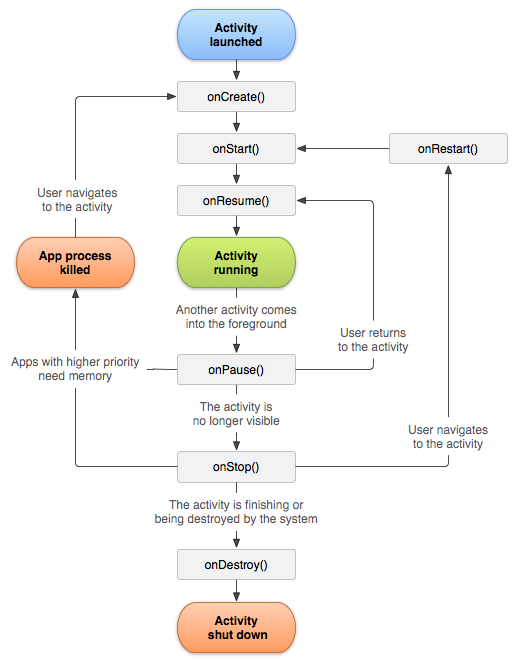
\includegraphics[width=0.6\linewidth]{pics/activity}
	\caption{activity}
	\label{fig:activity}
\end{figure}

Android использует специальный механизм описания действий основанный на Intent. Когда нужно выполнить действие (сделать звонок, послать письмо, показать окно), вызывается Intent.

Также Android содержит сервисы подобные демонам в Linux для выполнения нужных действий в фоновом режиме (например, проигрывание музыки).
Для обмена данными между приложениями используются Content providers (провайдеры содержимого).

Содержимое Activity формируется из различных компонентов, называемых View. Самые распространенные View - это кнопка, поле ввода, чекбокс и т.д. (рисунок~\ref{fig:view})

\begin{figure}[H]
	\centering
	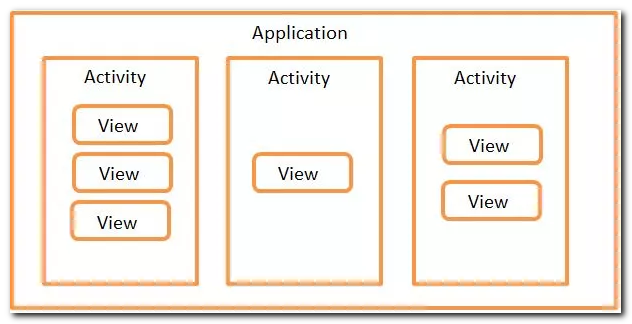
\includegraphics[width=0.6\linewidth]{pics/view}
	\caption{view}
	\label{fig:view}
\end{figure}

Необходимо заметить, что View обычно размещаются в ViewGroup. Самый распространенный пример ViewGroup – это Layout. Layout бывает различных типов и отвечает за то, как будут расположены его дочерние View на экране.

LinearLayout – отображает View-элементы в виде одной строки (если он Horizontal) или одного столбца (если он Vertical).

TableLayout – отображает элементы в виде таблицы, по строкам и столбцам.

RelativeLayout – для каждого элемента настраивается его положение относительно других элементов.

AbsoluteLayout – для каждого элемента указывается явная позиция на экране в системе координат (x,y)

\section{Основные компоненты пользовательского интерфейса мобильного приложения в Android}

В Android используется UI-фреймворк, сравнимый с другими полнофункциональными UI-фреймворками, применяемыми на локальных компьютерах. Он является более современным и асинхронным по природе. По существу, UI-фреймворк Android относится уже к четвертому поколению, если считать первым поколением традиционный прикладной интерфейс программирования Microsoft Windows, основанный на С, а MFC (Microsoft Foundation Classes, библиотека базовых классов Microsoft на основе C++) - вторым. В таком случае UI-фреймворк Swing, основанный на Java, будет третьим поколением, так как предлагаемые в нем возможности дизайна значительно превосходят по гибкости MFC. Android UI, JavaFX, Microsoft Silverlight и язык пользовательских интерфейсов Mozilla XML (XUL) относятся к новому типу UI-фреймворков четвертого поколения, в котором UI является декларативным и поддерживает независимую темизацию.

При программировании в пользовательском интерфейсе Android применяется объявление интерфейса в файлах XML. Затем эти определения представления (view definitions) XML загружаются в приложение с пользовательским интерфейсом как окна. Даже меню приложения загружаются из файлов XML. Экраны (окна) Android часто называются активностями (activities), которые включают в себя несколько видов, нужных пользователю, чтобы выполнить логический элемент процесса. Виды (views) являются основными элементами, из которых в Android состоит пользовательский интерфейс. Виды можно объединять в группы (view groups). Для внутренней организации видов используются давно известные в программировании концепции холст (canvas), рисование (painting) и взаимодействие пользователя с системой (user interaction).

Такие составные представления, в которые входят виды и группы видов, работают на базе специального логического заменяемого компонента пользовательского интерфейса Android.

Одной из ключевых концепций фреймворка Android является управление жизненным циклом (lifecycle) окон явлений (activity windows). В системе применяются протоколы, поэтому Android может управлять ситуацией по мере того, как пользователи скрывают, восстанавливают, останавливают и закрывают окна явлений.


\section{Проектирование структуры приложения}

Одна из важнейших задач в ходе создания мобильного приложения, преобразовывающего 2D снимки в объемные (3D) - разработка удобного и интуитивно-понятного пользовательского интерфейса. UI/UX (user Interface, user experience) составляющая, она же пользовательский интерфейс и пользовательский опыт, является более чем просто значимым элементом современного мобильного приложения. Удобство расположения элементов управления и приятное визуальное оформление напрямую влияют на настроение пользователя при использовании продукты. Именно некачественный UI/UX-дизайн отпугивает людей от использования многих приложений в пользу их более достойных альтернатив.

На главный экран камеры (рисунок~\ref{fig:Artboard}) выведены следующие функции:

\begin{itemize}
	\item Спуск затвора;
	\item Выбор фото из галереи;
	\item Смена камеры;
	\item Управление вспышкой;
	\item Переход к настройкам и справке.
\end{itemize}

\begin{figure}[H]
	\centering
	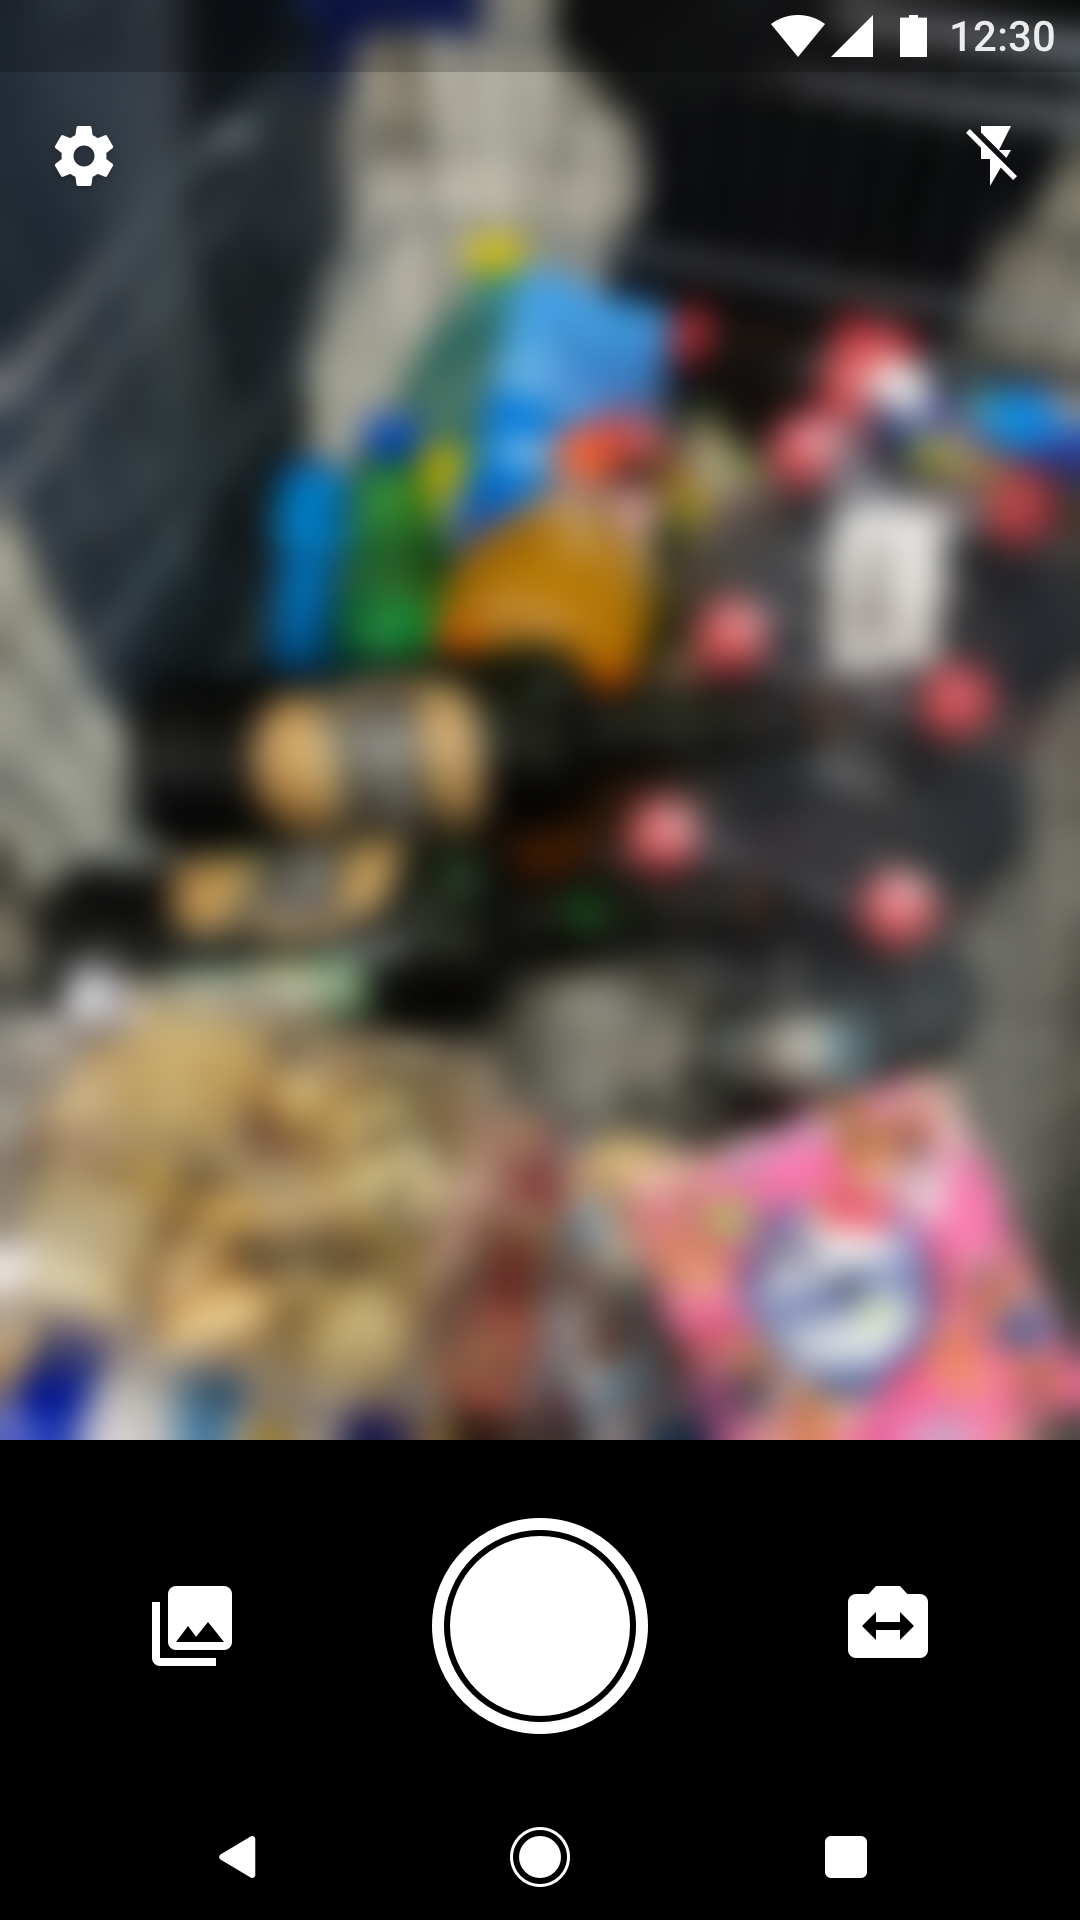
\includegraphics[width=0.6\linewidth]{pics/Artboard}
	\caption{Окно с камерой}
	\label{fig:Artboard}
\end{figure}

На экране с обработанной фотографией по нажатии кнопки «Далее» появляется bottom sheet (рисунок~\ref{fig:Artboard2}), включающий в себя быстрые функции шеринга и сохранения полученного фото в галерею.

\begin{figure}[H]
	\centering
	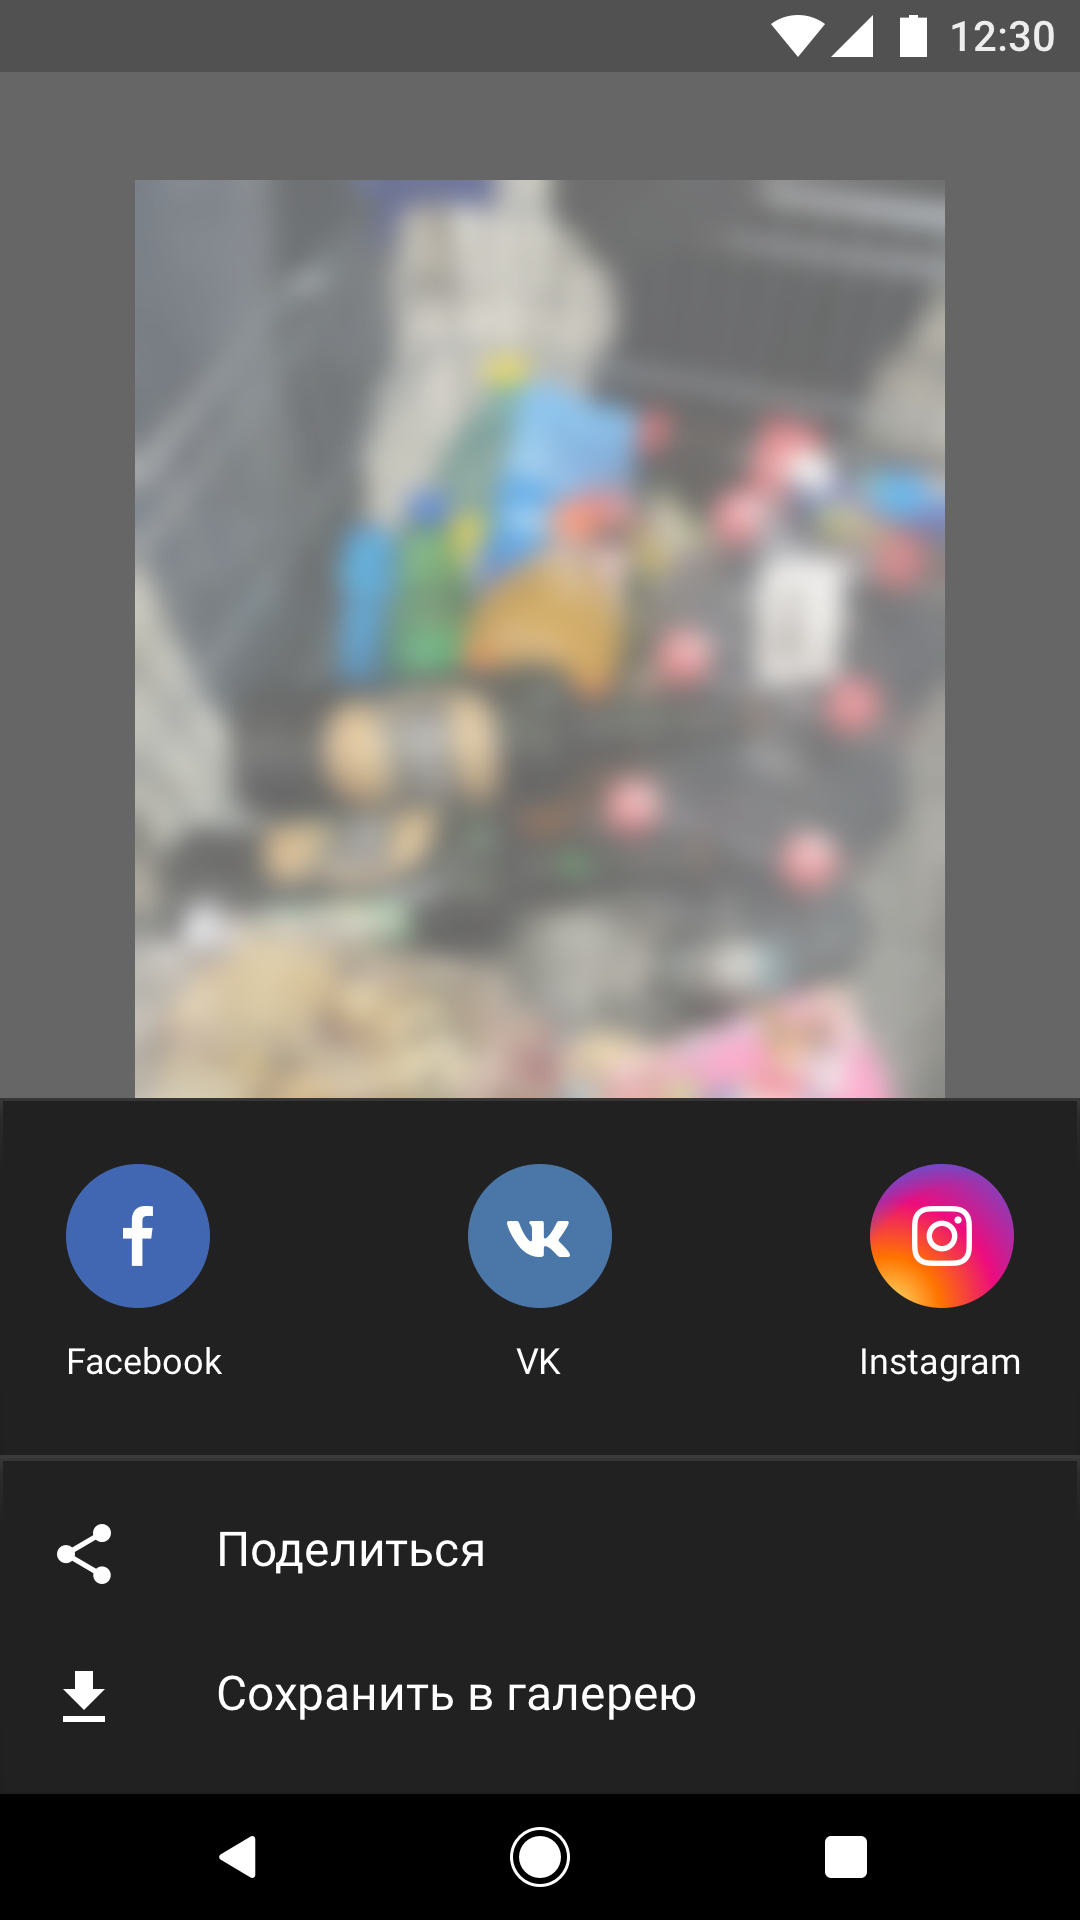
\includegraphics[width=0.6\linewidth]{pics/Artboard2}
	\caption{Окно с просмотром фото}
	\label{fig:Artboard2}
\end{figure}

При создании пользовательского интерфейса приложения были проанализированы современные, с аналогичным функционалом мобильные приложения в целом. Был сделан акцент на необходимости создания современного, функционального и не перегруженного пользовательского интерфейса. В результате проведенного анализа был создан пользовательский интерфейс мобильного приложения для преобразования 2D фотографий в 3D вид.

\section{Разработка мобильного приложения}

Рассмотрю практичный пример, когда программно запускаю приложение "Камера", а полученную фотографию сохраняю в папке.~\cite{camera}

В манифесте нужно добавить разрешение на запись файла в хранилище и указать требование наличия камеры.

Используем статическую константу ACTION\_IMAGE\_CAPTURE из объекта MediaStore для создания намерения, которое потом нужно передать методу startActivityForResult(). Разместим на форме кнопку и ImageView, в который будем помещать полученный снимок. Полученное с камеры изображение можно обработать в методе onActivityResult()

При тестировании примера на своём телефоне я обнаружил небольшую проблему - когда снимок передавался обратно на моё приложение, то оно находилось в альбомном режиме, а потом возвращалось в портретный режим. При этом полученный снимок терялся. Поэтому перед нажатием кнопки я поворачивал телефон в альбомный режим, чтобы пример работал корректно. Поэтому надо предусмотреть подобное поведение, например, запретить приложению реагировать на поворот и таким образом избежать перезапуска Activity. 

По умолчанию фотография возвращается в виде объекта Bitmap, содержащего миниатюру. Этот объект находится в параметре data, передаваемом в метод onActivityResult(). Чтобы получить миниатюру в виде объекта Bitmap, нужно вызвать метод getParcelableExtra() из намерения, передав ему строковое значение data.

(рисунок~\ref{fig:my})

\begin{figure}[H]
	\centering
	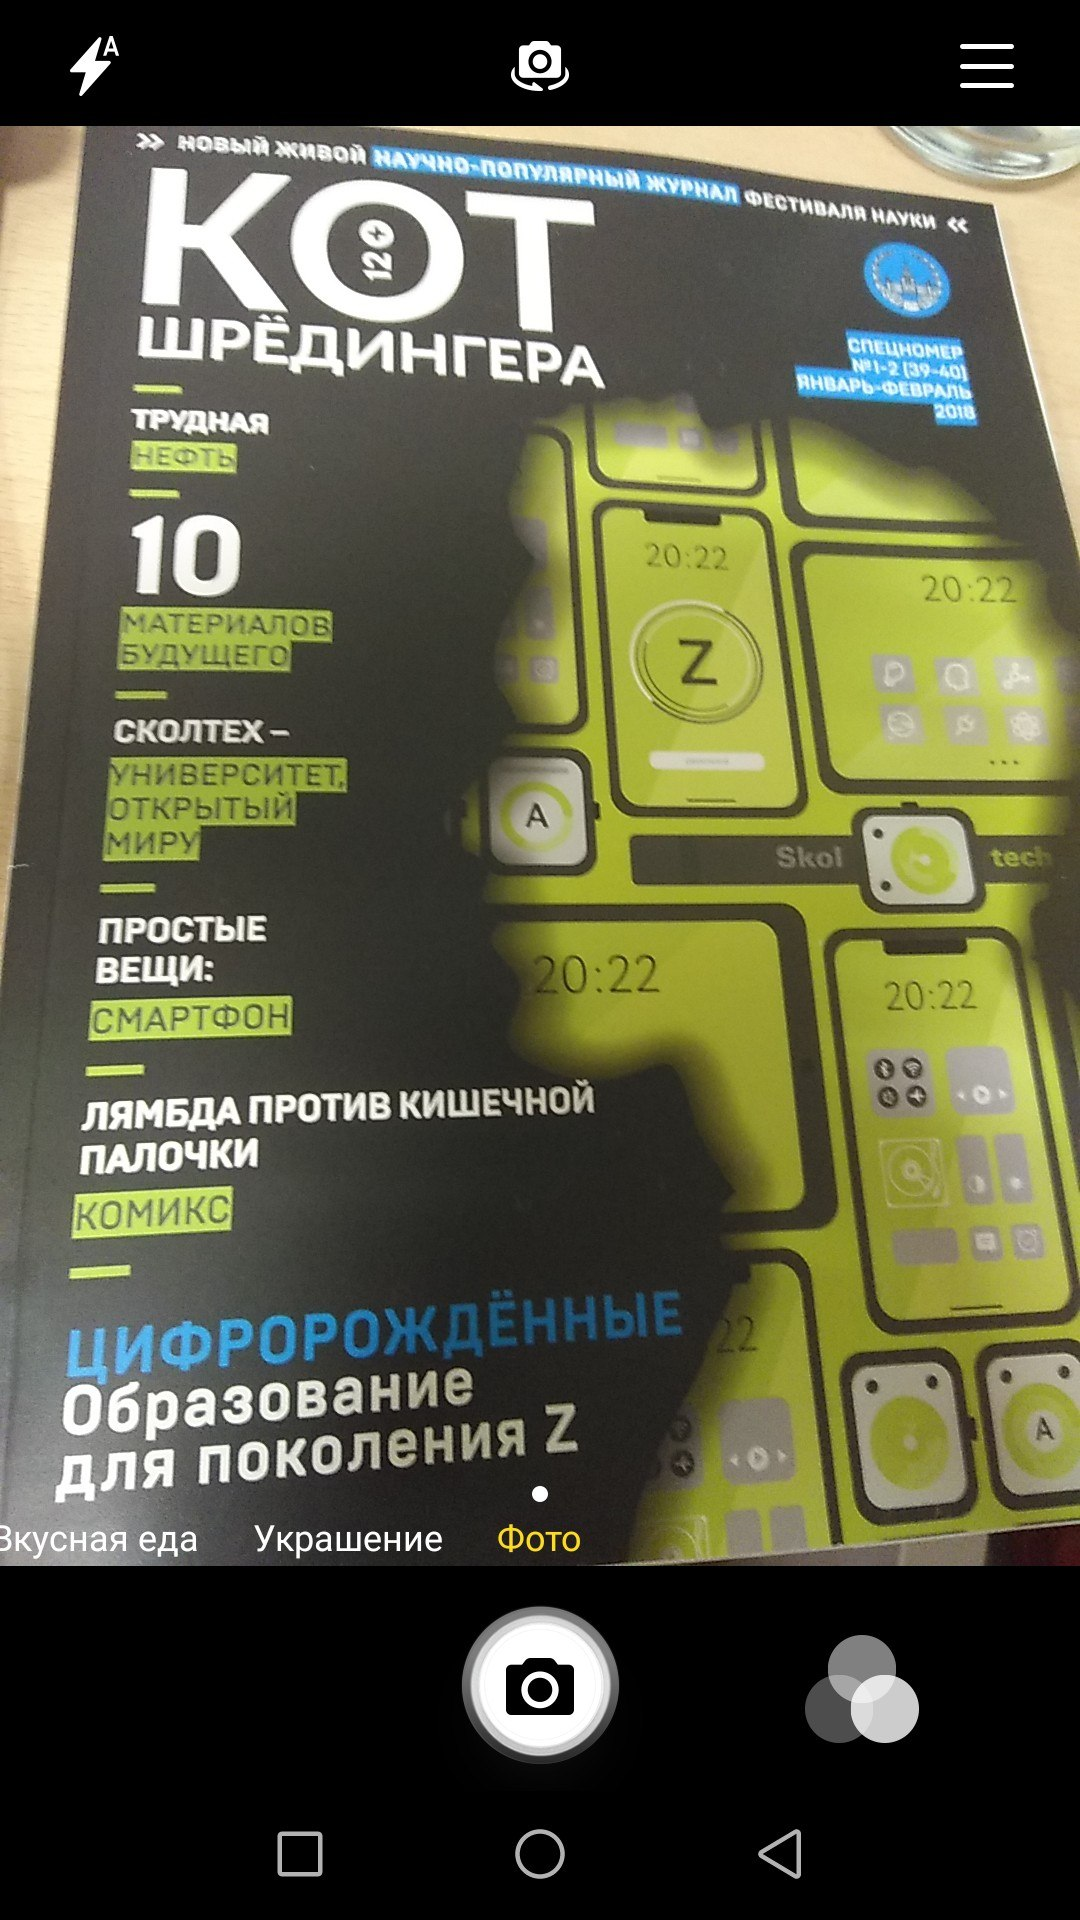
\includegraphics[width=0.4\linewidth]{pics/main}
	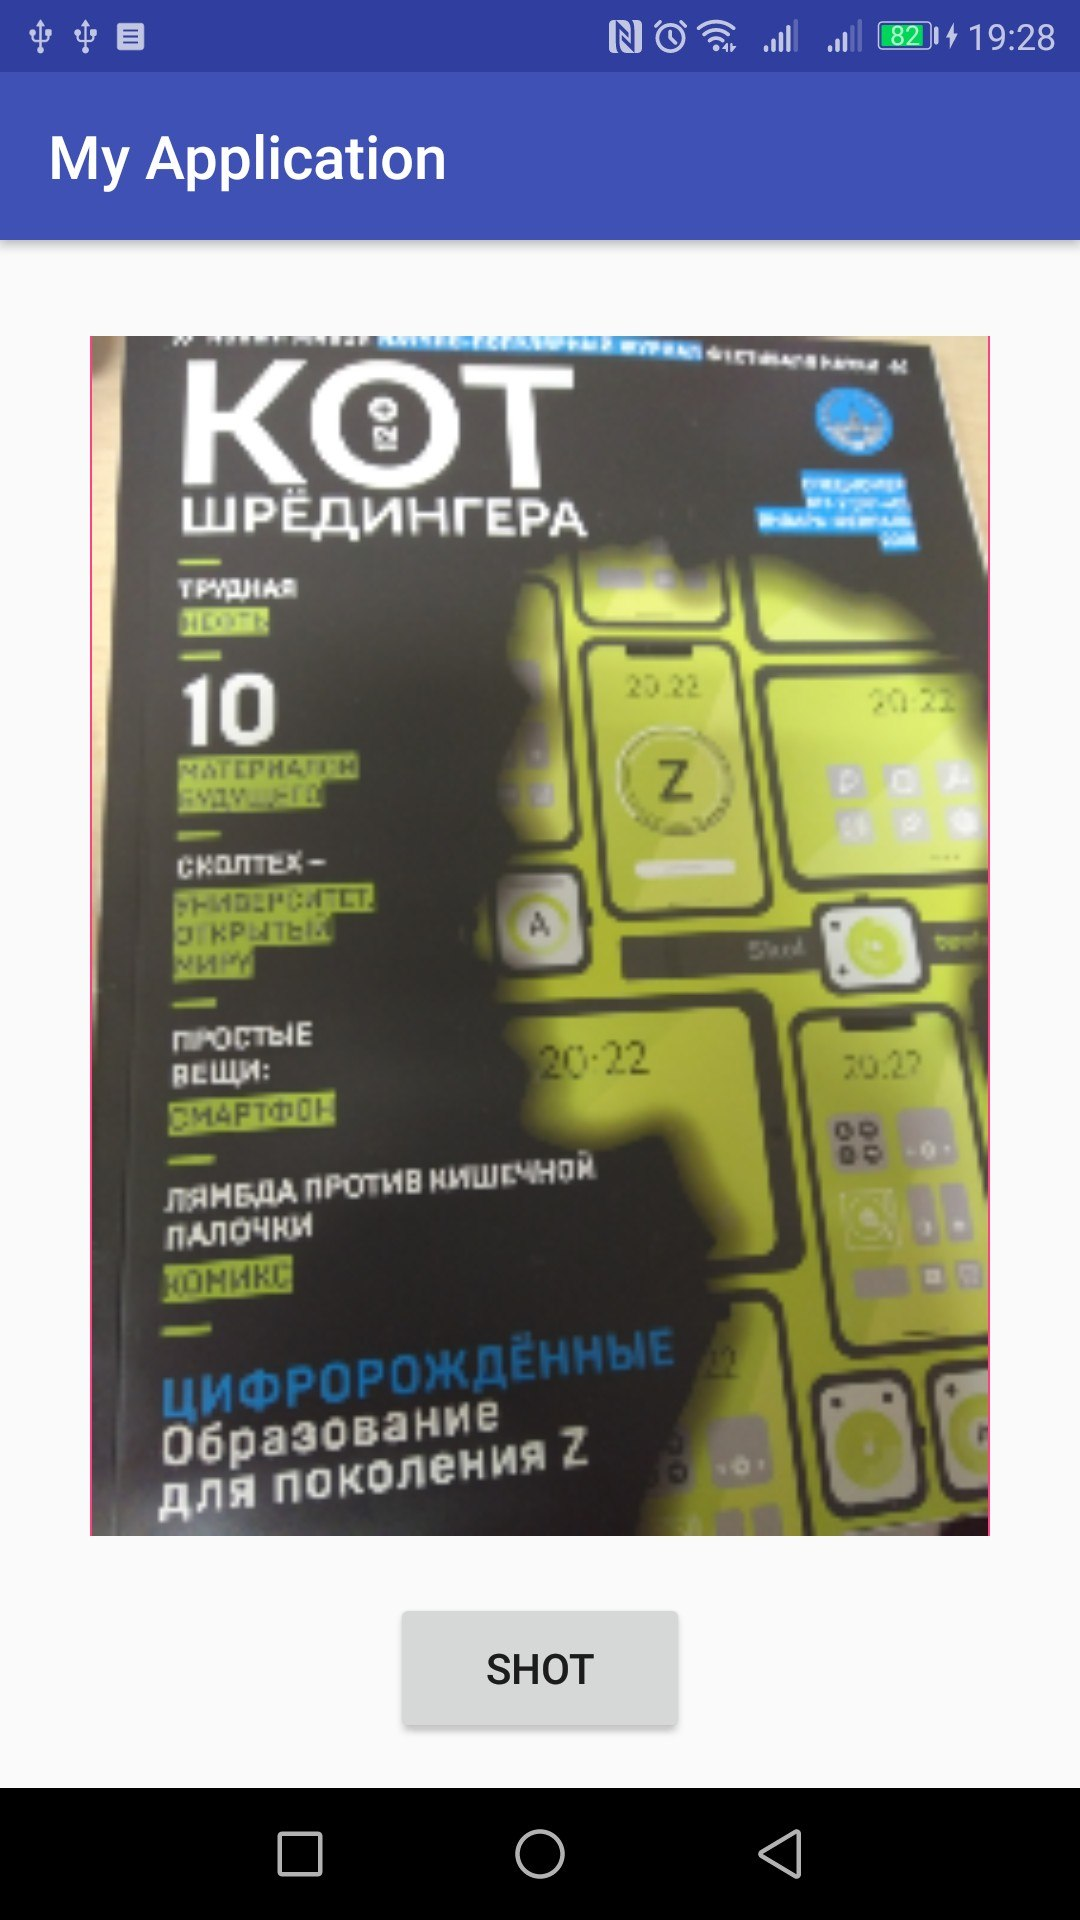
\includegraphics[width=0.4\linewidth]{pics/camera}
	\caption{Результат работы приложения}
	\label{fig:my}
\end{figure}
